% Informe final: celda 5G NR SA con USRP B210 (Comunicaciones Móviles, UNRC)
% Compilar desde informe/:  pdflatex informe_final.tex  (dos veces, para índice y referencias)
\documentclass[11pt,a4paper]{article}
\usepackage[T1]{fontenc}
\usepackage[utf8]{inputenc}
\usepackage[provide=*,spanish]{babel}
\usepackage{mathpazo}
\usepackage{microtype}
\usepackage[a4paper,margin=2.4cm]{geometry}
\usepackage{amsmath,amssymb}
\usepackage{graphicx}
\usepackage{booktabs,longtable,array,tabularx}
\usepackage{enumitem}
\usepackage[table]{xcolor}
\usepackage{caption}
\usepackage{tikz}
\usetikzlibrary{arrows.meta,positioning,fit,calc,shapes.geometric,backgrounds,decorations.pathreplacing}
\usepackage[hidelinks]{hyperref}
\usepackage{cleveref}

\captionsetup{font=small,labelfont=bf}
\AtBeginDocument{\renewcommand{\tablename}{Tabla}}
\crefname{figure}{figura}{figuras}
\crefname{table}{tabla}{tablas}
\crefname{section}{sección}{secciones}
\crefname{subsection}{sección}{secciones}
\crefname{equation}{ecuación}{ecuaciones}
\creflabelformat{equation}{(#2#1#3)}
\numberwithin{equation}{section}
\setlist{itemsep=2pt,topsep=4pt}
\setlength{\parskip}{3pt}

\definecolor{azul}{HTML}{2a78d6}
\definecolor{naranja}{HTML}{eb6834}
\definecolor{verde}{HTML}{1baf7a}
\definecolor{ocre}{HTML}{eda100}
\definecolor{gris}{HTML}{52514e}

% [verificar]: cita 3GPP que el grupo todavía no contrastó con el texto de la especificación
\newcommand{\verif}{\textbf{[verificar]}}
\newcommand{\ts}[1]{TS~#1}

\title{\textbf{Implementación de una celda 5G NR Standalone\\con una USRP B210}\\[4pt]
\large Informe final del trabajo práctico\\Comunicaciones Móviles --- Universidad Nacional de Río Cuarto}
\author{Grupo de trabajo 5G}
\date{Noviembre de 2026}

\begin{document}
\maketitle

\tableofcontents
\clearpage
\section{Consigna y objetivos}\label{sec:consigna}

\subsection{Consigna}
La consigna de la cátedra fue \emph{desplegar desde cero una celda 5G NR Standalone (opción~2, Release~15) en un entorno de RF controlado, lograr que un celular comercial con SIM de laboratorio se registre, obtenga una dirección IP y navegue, y medir throughput, latencia y jitter para compararlos con 2G (EDGE) y 4G (LTE)}. Además, se fijaron tres condiciones de método:
\begin{enumerate}
  \item toda la implementación (gNB, núcleo y base de datos) corre dentro de contenedores Docker;
  \item cada decisión de configuración se justifica con las especificaciones 3GPP, citando la TS y la sección;
  \item cada etapa (sincronización, acceso, registro, sesión PDU, tráfico IP y mediciones) se cierra con evidencia: logs, capturas o mediciones.
\end{enumerate}

\subsection{Objetivos}
\begin{itemize}
  \item \textbf{Objetivo general:} poner en servicio una celda NR SA funcional con hardware de radio definida por software y un teléfono comercial, y explicar su funcionamiento desde la capa física.
  \item \textbf{Objetivos específicos:}
  \begin{itemize}
    \item dimensionar la celda: banda, ancho de banda, numerología, cantidad de PRB, frecuencia de muestreo, patrón TDD y configuración del PRACH;
    \item preparar SIM de laboratorio que el teléfono acepte para 5G SA, y cargar los abonados en el núcleo;
    \item lograr el camino completo: sincronización, acceso aleatorio, registro, sesión PDU, IP y navegación;
    \item diagnosticar los problemas de estabilidad con la teoría de sincronización, acceso y control de enlace;
    \item medir throughput y latencia y contrastarlos con los máximos teóricos de TS~38.306;
    \item comparar CP-OFDM y DFT-s-OFDM en la subida.
  \end{itemize}
\end{itemize}

\subsection{Organización del informe}
Siguiendo las indicaciones de la cátedra, el informe empieza por la consigna; a continuación se resumen los resultados, y después se presentan 3GPP y los conceptos básicos (\cref{sec:marco}) y la numerología y los recursos de capa física (\cref{sec:numerologia}). Después trata primero el \emph{downlink}, empezando por las señales piloto que el teléfono busca al encenderse (\cref{sec:dl}), y luego el \emph{uplink} y los métodos de acceso (\cref{sec:ul}). La \cref{sec:flujos} calcula tamaños de bloque y tasas. Las \cref{sec:impl,sec:crono,sec:resultados} describen la implementación, el desarrollo cronológico y los resultados. La \cref{sec:preguntas} responde las preguntas de la cátedra con referencias a donde se desarrolla cada una.

Las citas a especificaciones marcadas como \verif{} no fueron contrastadas todavía con el texto de la norma. Las demás se comprobaron sobre el texto de las versiones Release~15 listadas en las referencias.

\section*{Resumen}\addcontentsline{toc}{section}{Resumen}
El grupo desplegó desde cero una celda 5G NR Standalone (opción~2, Release~15) con una USRP B210, el gNB OCUDU (ex srsRAN Project) y el núcleo Open5GS, todo dentro de contenedores Docker y en una jaula de Faraday. La celda principal opera en la banda n78 (TDD, 3525~MHz, 20~MHz, $\mu=1$, 51~PRB) con una frecuencia de muestreo de 23,04~MS/s, es decir, una FFT de 768~puntos a 30~kHz (equivalente a $1536\times 15$~kHz). También se puso en marcha una celda n3 FDD (1842,5/1747,5~MHz, 15~kHz, 106~PRB).

Un celular comercial (Xiaomi Redmi Note~14~5G) con una SIM de laboratorio programada por el grupo se registró en el núcleo, obtuvo una dirección IP y navegó por Internet a través de NAT. Para llegar a una conexión estable hubo que resolver cuatro problemas: el PLMN (con 722/999 los teléfonos no generaban PRACH; con el PLMN de prueba 001/01 se registraron al primer intento), el CSI que el teléfono no reportaba, una corrección de reloj que desplazaba la portadora sin corregir el muestreo y provocaba una deriva continua del \emph{timing advance}, y un corte del lado del teléfono cada 60~s, que se mitigó con el modo ``NR only'' y cuya relación con el anuncio de voz IMS sigue siendo una hipótesis.

Con la celda recién arrancada, la bajada TCP alcanzó $\approx 54$~Mbit/s (tasa del emisor), un 75~\% de la referencia aproximada de 71,7~Mbit/s que se obtiene de TS~38.306 para el patrón TDD usado. La subida llegó a 14,8~Mbit/s, contra una referencia de $\approx 35$~Mbit/s. El RTT mínimo fue de 16,7~ms y el mediano de 27,7~ms, aunque esta medición se hizo con la celda ya degradada. DFT-s-OFDM funcionó en la subida, pero no mejoró el rendimiento en este escenario de SINR alta. Eso es coherente con la teoría si el UE no estaba limitado en potencia, algo que queda como hipótesis porque no se registró el PHR. El informe desarrolla la teoría de capa física y de métodos de acceso que explica cada una de estas observaciones.

\section{Marco teórico: 3GPP y conceptos básicos de 5G NR}\label{sec:marco}

\subsection{3GPP y las releases}
El 3GPP (\emph{3rd Generation Partnership Project}) agrupa a los organismos regionales de normalización y publica las especificaciones técnicas (TS) de los sistemas móviles. Cada TS se identifica por serie: la serie~38 corresponde a la red de acceso NR, la~23 a la arquitectura del sistema, la~24 a los protocolos con el terminal (NAS), la~31 a la tarjeta (U)SIM y la~33/35 a la seguridad y sus algoritmos. Las especificaciones evolucionan por \emph{releases}, y cada una congela un conjunto coherente de funciones:
\begin{itemize}
  \item \textbf{Release~15:} primera release de 5G NR. Definió primero la operación no autónoma (NSA, anclada en LTE) y después la autónoma (SA), con el núcleo 5GC. Es la release que pide la consigna.
  \item \textbf{Release~16:} mejoras para comunicaciones de baja latencia y alta confiabilidad (URLLC), IoT industrial, V2X y NR en espectro sin licencia.
  \item \textbf{Release~17:} terminales de capacidad reducida (RedCap), redes no terrestres y extensión de frecuencias.
  \item \textbf{Release~18:} primera release de \emph{5G-Advanced}.
\end{itemize}
La capa física que se describe en este informe es la de Release~15 (TS~38.211, 38.212, 38.213 y 38.214), que es la que implementan el gNB usado y los teléfonos.

\subsection{NSA contra SA}
En la opción~3 (NSA, también llamada EN-DC) el teléfono se conecta a la vez a un eNB LTE, que actúa como ancla de control, y a un gNB que aporta capacidad de datos. El núcleo sigue siendo el EPC de LTE. En la \textbf{opción~2 (SA)}, en cambio, el gNB se conecta directamente al núcleo 5G (5GC) y toda la señalización (RRC y NAS) viaja por NR \cite{ts38300}. Para este trabajo SA tiene dos consecuencias prácticas:
\begin{enumerate}
  \item el teléfono tiene que encontrar, sincronizarse y acampar en la celda NR sin ayuda de LTE, así que el SSB, el MIB y el SIB1 tienen que estar bien configurados (\cref{sec:dl});
  \item hace falta un núcleo 5GC completo, y el teléfono tiene que aceptar la SIM para el acceso NG-RAN (\cref{sec:impl}).
\end{enumerate}

\subsection{Arquitectura: gNB y 5GC}
La \cref{fig:arquitectura} (en la \cref{sec:impl}) muestra la arquitectura implementada. Solo se describen las funciones necesarias para seguir el informe \cite{ts38300}:
\begin{itemize}
  \item \textbf{gNB:} termina la interfaz radio (PHY, MAC, RLC, PDCP, SDAP y RRC). En el gNB usado, las funciones se dividen en CU y DU, pero corren en un mismo proceso.
  \item \textbf{AMF} (\emph{Access and Mobility Management Function}): termina la señalización NAS del UE (registro, autenticación, movilidad) y la interfaz \textbf{N2} con el gNB (protocolo NGAP sobre SCTP).
  \item \textbf{SMF} (\emph{Session Management Function}): gestiona las sesiones PDU (asignación de IP, DNN) y controla al UPF.
  \item \textbf{UPF} (\emph{User Plane Function}): reenvía el tráfico de usuario. Lo recibe del gNB por la interfaz \textbf{N3} (túneles GTP-U sobre UDP) y lo entrega a la red de datos por \textbf{N6}. En este trabajo, N6 termina en la NAT del kernel Linux, que da salida a Internet.
  \item \textbf{AUSF, UDM y UDR:} autentican al abonado con 5G-AKA y guardan sus credenciales. En Open5GS, el UDR usa MongoDB.
\end{itemize}

\subsection{Rangos de frecuencia y bandas usadas}
NR define dos rangos de frecuencia: \textbf{FR1} (por debajo de 7,125~GHz) y \textbf{FR2} (ondas milimétricas, desde 24,25~GHz) \cite[tabla~5.1-1]{ts38101}: en la versión 15.31.0, FR1 va de 410 a 7125~MHz y FR2, de 24\,250 a 52\,600~MHz. Este trabajo usa dos bandas de FR1:
\begin{itemize}
  \item \textbf{n78} (3300--3800~MHz, TDD): la banda media típica de 5G. En TDD, la subida y la bajada comparten la misma portadora y se alternan en el tiempo según un patrón de slots (\cref{sec:tdd}). Admite SCS de 15, 30 y 60~kHz para datos.
  \item \textbf{n3} (subida 1710--1785~MHz, bajada 1805--1880~MHz, FDD): la banda de 1800~MHz heredada de 2G y 4G. En FDD, la subida y la bajada usan portadoras distintas separadas 95~MHz y transmiten en simultáneo.
\end{itemize}

La frecuencia de una portadora se expresa con el NR-ARFCN $N_\text{REF}$, según \cite[§5.4.2.1]{ts38101}:
\begin{equation}
F_\text{REF} = F_\text{REF-Offs} + \Delta F_\text{Global}\,(N_\text{REF}-N_\text{REF-Offs}),
\label{eq:arfcn}
\end{equation}
con $\Delta F_\text{Global}=5$~kHz y $F_\text{REF-Offs}=0$ por debajo de 3~GHz, y $\Delta F_\text{Global}=15$~kHz, $F_\text{REF-Offs}=3000$~MHz y $N_\text{REF-Offs}=600\,000$ entre 3 y 24,25~GHz. Para la celda n78, $N_\text{REF}=635\,000$ da $3000 + 0{,}015\cdot 35\,000 = 3525$~MHz. Para la n3, $N_\text{REF}=368\,500$ da $0{,}005\cdot 368\,500=1842{,}5$~MHz en la bajada y, con la separación dúplex de 95~MHz, 1747,5~MHz en la subida.

\section{Capa física: numerología y recursos}\label{sec:numerologia}

\subsection{Numerología: \texorpdfstring{$\mu$}{mu}, SCS, slots y símbolos}
A diferencia del LTE convencional, que usa para los datos una única separación entre subportadoras de 15~kHz, NR admite una familia de numerologías escaladas por potencias de dos \cite[§4.2]{ts38211}:
\begin{equation}
\Delta f = 2^{\mu}\cdot 15~\text{kHz}, \qquad \mu \in \{0,1,2,3,4\}.
\label{eq:scs}
\end{equation}
La trama dura siempre 10~ms y se divide en 10 subtramas de 1~ms. Cada subtrama tiene $2^\mu$ slots, y cada slot, 14 símbolos OFDM con CP normal \cite[§4.3.1, tabla~4.3.2-1]{ts38211}. Por lo tanto, al duplicar la SCS se reduce a la mitad la duración del símbolo y del slot (\cref{tab:numerologia}).

\begin{table}[htbp]
\centering
\caption{Numerologías de NR con CP normal (TS~38.211, tablas 4.2-1 y 4.3.2-1). La duración del CP es la de los símbolos comunes; el primero de cada medio subtrama tiene $16\kappa T_c = 0{,}52~\mu$s más.}
\label{tab:numerologia}
\begin{tabular}{cccccc}
\toprule
$\mu$ & $\Delta f$ [kHz] & slots/trama & slot [ms] & símbolo útil [$\mu$s] & CP [$\mu$s] \\
\midrule
0 & 15 & 10 & 1 & 66,67 & 4,69 \\
\rowcolor{azul!10} 1 & 30 & 20 & 0,5 & 33,33 & 2,34 \\
2 & 60 & 40 & 0,25 & 16,67 & 1,17 \\
3 & 120 & 80 & 0,125 & 8,33 & 0,59 \\
4 & 240 & 160 & 0,0625 & 4,17 & 0,29 \\
\bottomrule
\end{tabular}
\end{table}

La celda n78 usa $\mu=1$ (30~kHz): un slot dura 0,5~ms y hay 20 slots por trama. El símbolo útil dura $T_u = 1/\Delta f = 33{,}33~\mu$s. La celda n3 usa $\mu=0$, como LTE.

La elección de la numerología es un compromiso: una SCS mayor acorta el símbolo, lo que reduce la latencia y da más tolerancia al Doppler y al ruido de fase, pero también acorta el CP, lo que reduce la tolerancia al ensanchamiento temporal del canal (\cref{sec:cp}). En n78, 30~kHz es el valor típico de banda media.

\subsection{Unidad de tiempo \texorpdfstring{$T_c$}{Tc} y frecuencia de muestreo}\label{sec:fs}
TS~38.211 define todas las duraciones como múltiplos de una unidad básica \cite[§4.1]{ts38211}:
\begin{equation}
T_c = \frac{1}{\Delta f_\text{max}\cdot N_f} = \frac{1}{480\cdot 10^3~\text{Hz}\cdot 4096} \approx 0{,}509~\text{ns},
\label{eq:tc}
\end{equation}
que corresponde a la mayor SCS prevista (480~kHz) con una FFT de 4096 puntos. La relación con la unidad de LTE, $T_s = 1/(15~\text{kHz}\cdot 2048) = 32{,}55$~ns, es la constante
\begin{equation}
\kappa = \frac{T_s}{T_c} = 64.
\label{eq:kappa}
\end{equation}
La ``frecuencia de muestreo básica'' de NR es entonces $1/T_c = 1{,}966\,08$~GHz. \textbf{No es la frecuencia a la que muestrea un equipo real:} es una grilla temporal común que permite escribir todas las duraciones de todas las numerologías como números enteros. Un transmisor real muestrea a
\begin{equation}
f_s = N_\text{FFT}\cdot \Delta f,
\label{eq:fs}
\end{equation}
donde $N_\text{FFT}$ es el tamaño de la IFFT/FFT elegido por la implementación. La condición básica es que $N_\text{FFT}$ sea mayor que la cantidad de subportadoras ocupadas, para que la señal compleja en banda base quepa en $[-f_s/2, f_s/2)$ con margen para los filtros; en la práctica también influyen los relojes que admite el hardware y el costo de la FFT.

\paragraph{Frecuencia de muestreo de la celda.} La B210 se configuró a $f_s = 23{,}04$~MS/s:
\begin{equation}
f_s = 1536\cdot 15~\text{kHz} = 768\cdot 30~\text{kHz} = 23{,}04~\text{MHz}.
\label{eq:fs_celda}
\end{equation}
\begin{itemize}
  \item En n78 ($\Delta f = 30$~kHz) la FFT es de 768 puntos, y en n3 ($\Delta f=15$~kHz), de 1536 puntos. En ambos casos, el ancho de banda de muestreo es el mismo: $1536\times 15~\text{kHz}$.
  \item Hay 612 subportadoras ocupadas en n78 (51~PRB $\times$ 12) y 1272 en n3 (106~PRB $\times$ 12): ambas entran en la FFT, con un factor de sobremuestreo de $768/612 \approx 1{,}25$ y $1536/1272\approx 1{,}21$.
  \item $768 = 2^8\cdot 3$ y $1536 = 2^9\cdot 3$ no son potencias de dos, pero se calculan eficientemente con FFT de base mixta. La alternativa de potencia de dos inmediata (1024 puntos a 30~kHz) exige 30,72~MS/s.
  \item 23,04~MS/s es una elección compatible y eficiente para 20~MHz en esta plataforma, no un mínimo universal. Con el formato \texttt{sc12} (12 bits por componente, 3 bytes por muestra compleja) el flujo es de $23{,}04\cdot 10^6\cdot 3 \approx 69$~MB/s en cada sentido. Ese caudal solo es sostenible por USB~3.0, lo que explica el primer problema práctico de la \cref{sec:crono}.
\end{itemize}

\Cref{tab:fs} compara las frecuencias de muestreo posibles para $\mu=1$. Las duraciones en muestras salen de multiplicar las de la norma ($2048\kappa 2^{-\mu} = 65\,536$, $144\kappa 2^{-\mu} = 4608$ y $144\kappa 2^{-\mu}+16\kappa = 5632$, en unidades de $T_c$) por $f_s T_c$. Por ejemplo, a 23,04~MS/s, $f_s T_c = 23{,}04/1966{,}08 = 3/256$.

\begin{table}[htbp]
\centering
\caption{Muestras por símbolo y por slot para $\mu=1$ según la frecuencia de muestreo. En todas, un slot dura 0,5~ms.}
\label{tab:fs}
\begin{tabular}{lcccc}
\toprule
$f_s$ & $N_\text{FFT}$ & CP normal & CP largo (1.\textsuperscript{er} símbolo) & muestras por slot \\
\midrule
\rowcolor{azul!10} 23,04 MS/s (usada) & 768 & 54 & 66 & $768\cdot14+54\cdot13+66 = 11\,520$ \\
30,72 MS/s & 1024 & 72 & 88 & 15\,360 \\
61,44 MS/s & 2048 & 144 & 176 & 30\,720 \\
1,966 GHz ($1/T_c$) & 65\,536 & 4608 & 5632 & 983\,040 \\
\bottomrule
\end{tabular}
\end{table}

La comprobación para la frecuencia usada es directa: $11\,520 / 23{,}04~\text{MS/s} = 0{,}5$~ms. El CP vale $54/23{,}04~\text{MHz} = 2{,}344~\mu$s y el largo, $66/23{,}04~\text{MHz} = 2{,}865~\mu$s, idénticos a los de TS~38.211.

\subsection{Grilla de recursos, RE y PRB}
El recurso elemental es el \textbf{resource element} (RE): una subportadora durante un símbolo OFDM. Un \textbf{PRB} agrupa 12 subportadoras consecutivas en frecuencia \cite[§4.4]{ts38211}. A diferencia de LTE, en NR el PRB se define solo en frecuencia: en el tiempo, la unidad de planificación es el slot o una fracción de él (asignaciones de 2 a 14 símbolos). Con $\mu=1$, un PRB ocupa $12\cdot 30 = 360$~kHz.

Todas las grillas se referencian al \textbf{punto A}, una frecuencia común a todas las numerologías. A partir de él se numeran los CRB (\emph{common resource blocks}), y una \emph{bandwidth part} (BWP) es un subconjunto contiguo de CRB con una numerología dada. En esta celda hay una sola BWP, que ocupa los 51~PRB del canal.

\subsection{Cálculo de PRB y de banda de guarda}\label{sec:guarda}
TS~38.101-1 fija, para cada ancho de banda de canal y SCS, la cantidad máxima de PRB $N_\text{RB}$ (tabla~5.3.2-1) y la banda de guarda mínima a cada lado (tabla~5.3.3-1) \cite{ts38101}\verif. La banda de guarda mínima se obtiene de
\begin{equation}
G_\text{BW} = \frac{\text{BW}_\text{canal} - N_\text{RB}\cdot 12\cdot\Delta f}{2} - \frac{\Delta f}{2},
\label{eq:guarda}
\end{equation}
donde el término $\Delta f/2$ tiene en cuenta que la grilla de subportadoras está desplazada media subportadora respecto del centro del canal.

\paragraph{n78, 20~MHz, 30~kHz ($N_\text{RB}=51$).}
\begin{align}
\text{BW ocupado} &= 51\cdot 12\cdot 30~\text{kHz} = 18\,360~\text{kHz} \quad (91{,}8~\%\text{ del canal}),\\
G_\text{BW} &= \frac{20\,000-18\,360}{2} - \frac{30}{2} = 820 - 15 = 805~\text{kHz}.
\end{align}

\paragraph{n3, 20~MHz, 15~kHz ($N_\text{RB}=106$).}
\begin{align}
\text{BW ocupado} &= 106\cdot 12\cdot 15~\text{kHz} = 19\,080~\text{kHz} \quad (95{,}4~\%),\\
G_\text{BW} &= \frac{20\,000-19\,080}{2} - 7{,}5 = 460 - 7{,}5 = 452{,}5~\text{kHz}.
\end{align}

Con 15~kHz se aprovecha mejor el canal (95,4~\% contra 91,8~\%) porque la guarda que necesitan los filtros es, en proporción, menor. LTE, con 100~PRB en 20~MHz, ocupaba solo el 90~\%. La guarda protege a los canales adyacentes de la emisión fuera de banda: los lóbulos laterales de las subportadoras OFDM decaen lentamente (como una sinc) y el filtrado o el \emph{windowing} necesita una banda de transición.

\subsection{Prefijo cíclico}\label{sec:cp}
\subsubsection{Función del CP}
El canal multitrayecto tiene una respuesta al impulso de duración $\tau_\text{max}$ (\emph{delay spread}). Si se antepone a cada símbolo una copia de sus últimas $N_\text{CP}$ muestras, con $T_\text{CP}\ge\tau_\text{max}$:
\begin{enumerate}
  \item la interferencia entre símbolos (ISI) queda confinada al CP, que el receptor descarta;
  \item la convolución lineal con el canal se vuelve \textbf{circular} dentro de la ventana de la FFT, así que cada subportadora ve una ganancia compleja $H_k$ y se ecualiza con un solo coeficiente, sin interferencia entre portadoras (ICI).
\end{enumerate}
Por eso, \textbf{el valor mínimo del prefijo cíclico es el delay spread del canal} (más el error residual de sincronización):
\begin{equation}
T_\text{CP} \ge \tau_\text{max}.
\label{eq:cpmin}
\end{equation}
El costo es la eficiencia: el CP no lleva información nueva, así que se pierde una fracción $T_\text{CP}/(T_u + T_\text{CP})$ del tiempo y de la energía.

\subsubsection{Ejercicio planteado por la cátedra}\label{sec:ejercicio_cp}
Se supone un delay spread igual a un cuarto del símbolo útil, con $\Delta f=15$~kHz:
\begin{equation}
\tau = \frac{1}{4\,\Delta f} = \frac{1}{4\cdot 15~\text{kHz}} = 16{,}67~\mu\text{s}.
\end{equation}
Con $f_s = 1536\cdot 15~\text{kHz} = 23{,}04$~MHz, el período de muestreo es
\begin{equation}
T_s = \frac{1}{f_s} = \frac{1}{23{,}04~\text{MHz}} = 43{,}40~\text{ns},
\end{equation}
y el CP necesario, en muestras,
\begin{equation}
N_\text{CP} = \frac{\tau}{T_s} = \frac{16{,}67~\mu\text{s}}{43{,}40~\text{ns}} = 384~\text{muestras}.
\end{equation}
Sumadas a las 1536 muestras de la IFFT, el símbolo completo tiene $1536+384 = 1920$ muestras, y dura
\begin{equation}
T_\text{símb} = \frac{1920}{23{,}04~\text{MHz}} = 83{,}33~\mu\text{s} = 66{,}67~\mu\text{s (útil)} + 16{,}67~\mu\text{s (CP)}.
\end{equation}
Con una IFFT de 2048 puntos ($f_s = 30{,}72$~MHz) el CP sería de 512 muestras: cambia la cantidad de muestras, pero no la duración del símbolo, que depende solo de $\Delta f$ y de la fracción de CP. Catorce símbolos de este tipo duran $14\cdot 83{,}33~\mu\text{s} = 1{,}167$~ms.

\subsubsection{Comparación con NR}
Con un CP de $T_u/4$ no entran 14 símbolos en 1~ms, sino
\begin{equation}
\left\lfloor \frac{1~\text{ms}}{83{,}33~\mu\text{s}} \right\rfloor = 12~\text{símbolos}.
\end{equation}
Ese es exactamente el caso del \textbf{CP extendido}: en LTE, $512$ muestras a 30,72~MHz (16,67~$\mu$s) y 12 símbolos por subtrama. En NR, el CP extendido solo existe para $\mu=2$ ($512\kappa 2^{-\mu}T_c$) \cite[§5.3.1]{ts38211}.

El \textbf{CP normal} de NR es mucho más corto. Según TS~38.211 §5.3.1,
\begin{equation}
N_{\text{CP},l}^{\mu} =
\begin{cases}
144\kappa\, 2^{-\mu} + 16\kappa & l = 0 \text{ o } l = 7\cdot 2^{\mu}\\
144\kappa\, 2^{-\mu} & \text{en otro caso}
\end{cases}
\qquad[\text{en unidades de } T_c].
\label{eq:ncp}
\end{equation}
Para $\mu=0$, a 30,72~MHz, son 144 muestras (4,69~$\mu$s), y 160 en el primer símbolo de cada medio subframe. Así entran 14 símbolos en 1~ms:
\begin{equation}
2048\cdot 14 + 144\cdot 14 + 16\cdot 2 = 28\,672 + 2016 + 32 = 30\,720~\text{muestras} = 1~\text{ms}\times 30{,}72~\text{MS/s}.
\end{equation}
Para la celda n3, a 23,04~MHz con FFT de 1536, la misma cuenta da $1536\cdot 14 + 108\cdot 14 + 12\cdot 2 = 23\,040$ muestras. Para la celda n78 ($\mu=1$), el CP normal es de $144\cdot 64\cdot 2^{-1}\,T_c = 2{,}344~\mu$s, y de $2{,}865~\mu$s en el primer símbolo de cada slot.

\textbf{Importante:} en NR, los 14 símbolos forman un \textbf{slot}, no una trama. La trama dura siempre 10~ms; según la numerología contiene entre 10 y 160 slots (\cref{tab:numerologia}).

\paragraph{Delay spread tolerable.} Un CP de $2{,}344~\mu$s cubre trayectos que difieren hasta
\begin{equation}
\Delta d = c\cdot T_\text{CP} = 3\cdot 10^8~\text{m/s}\cdot 2{,}344\cdot 10^{-6}~\text{s} \approx 703~\text{m}.
\end{equation}
Es más que suficiente para una jaula de Faraday o un ambiente de interiores (delay spreads de decenas a cientos de nanosegundos), y razonable para microceldas urbanas. Con 15~kHz, el CP de 4,69~$\mu$s tolera $\approx 1{,}4$~km.

\subsection{Estructura TDD}\label{sec:tdd}
En TDD, el gNB difunde en el SIB1 el patrón de slots \texttt{tdd-UL-DL-ConfigurationCommon} \cite[§11.1]{ts38213}. En la celda n78, ese patrón tiene un período de 5~ms (10 slots) y es \texttt{DDDDDDSUUU} (\cref{fig:tdd}):
\begin{itemize}
  \item 6 slots de bajada (D);
  \item 1 slot especial (S) con 8 símbolos de bajada, 0 de subida y 6 de guarda;
  \item 3 slots de subida (U).
\end{itemize}
El \textbf{período de guarda} cubre el tiempo de conmutación del hardware y el retardo de ida y vuelta: el UE tiene que terminar de recibir la bajada y adelantar su transmisión en el \emph{timing advance} (\cref{sec:ta}) sin que la subida se superponga con la bajada siguiente.

\begin{figure}[htbp]
\centering
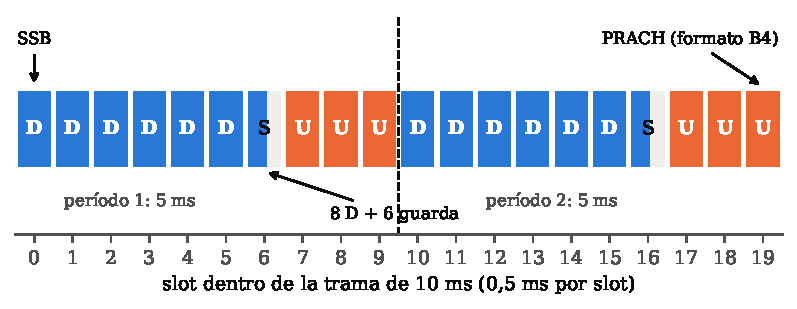
\includegraphics[width=\linewidth]{figuras/fig_tdd.pdf}
\caption{Patrón TDD de la celda n78 en una trama de 10~ms: dos períodos de 5~ms \texttt{DDDDDDSUUU}. El SSB va en el slot~0 y la ocasión de PRACH (formato B4, índice 159), en el slot~19.}
\label{fig:tdd}
\end{figure}

Las fracciones de símbolos por sentido en un período son:
\begin{align}
\text{DL:}\quad & \frac{6\cdot 14 + 8}{10\cdot 14} = \frac{92}{140} = 0{,}657, \label{eq:fdl}\\
\text{UL:}\quad & \frac{3\cdot 14}{140} = \frac{42}{140} = 0{,}30, \label{eq:ful}\\
\text{guarda:}\quad & \frac{6}{140} = 0{,}043.
\end{align}
Estas fracciones limitan el throughput de cada sentido (\cref{sec:tput}) y fijan cuánto hay que esperar un slot de subida (\cref{sec:latencia}).

\section{Downlink}\label{sec:dl}

El downlink se trata primero porque es lo primero que el teléfono necesita: antes de poder transmitir, tiene que encontrar la celda, sincronizarse en tiempo y frecuencia y leer la información de sistema. Todo eso lo consigue con las señales piloto que el gNB difunde de manera permanente.

\subsection{Qué pasa al prender el celular}\label{sec:encendido}
Al encenderse, el teléfono no sabe en qué frecuencia está la celda, cuál es su numerología, cuándo empieza la trama ni cuál es su identidad. La búsqueda inicial sigue estos pasos: la sincronización está en TS~38.213 §4.1 \cite{ts38213}, la selección de PLMN y de celda en TS~23.122 y TS~38.304 \cite{ts23122,ts38304}, y la información de sistema en TS~38.331 \cite{ts38331}:
\begin{enumerate}
  \item \textbf{Selección de PLMN y bandas.} Con la lista de PLMN y tecnologías de acceso de la SIM y las bandas que soporta el módem, el teléfono decide qué bandas barrer. Por eso la programación de la SIM resultó decisiva (\cref{sec:crono}).
  \item \textbf{Barrido sobre el \emph{sync raster}.} En lugar de probar cada posición posible del canal (el \emph{channel raster} de 15 o 30~kHz), el UE busca el SSB solo en las frecuencias del \emph{synchronization raster}, numeradas con el GSCN (\cref{sec:gscn}).
  \item \textbf{Detección del PSS.} En cada candidato, el UE correlaciona la señal recibida con las 3 secuencias PSS posibles. Un pico de correlación le da la temporización de símbolo, una estimación gruesa del desvío de frecuencia (CFO) y $N_\text{ID}^{(2)}$.
  \item \textbf{Detección del SSS.} Con la temporización ya fijada, el UE prueba las 336 hipótesis de $N_\text{ID}^{(1)}$ y obtiene el PCI.
  \item \textbf{PBCH.} Con el PCI, el UE conoce la DM-RS del PBCH, estima el canal y decodifica el MIB, que tiene código polar y CRC. Así obtiene el número de trama (SFN), el medio de trama y el índice del SSB, y queda sincronizado a la trama.
  \item \textbf{SIB1.} El MIB indica dónde están el CORESET~0 y el espacio de búsqueda~0. Ahí el UE busca un PDCCH con el SI-RNTI, que planifica el PDSCH con el SIB1. El SIB1 lleva el PLMN, el TAC, el criterio de selección de celda, la configuración TDD, la del PRACH y la potencia del SSB.
  \item \textbf{Selección de celda y acampe.} Si el PLMN es aceptable, la celda no está bloqueada y el nivel recibido supera \texttt{q-RxLevMin}, el UE acampa y puede iniciar el acceso aleatorio (\cref{sec:rach}).
\end{enumerate}
Para la búsqueda inicial, el UE supone que el SSB se repite cada 20~ms \cite[§4.1]{ts38213}. En esta celda se transmite cada 10~ms (\texttt{ssb-PeriodicityServingCell = ms10}), así que el UE ve dos ráfagas en cada ventana.

\subsubsection{Raster de sincronización y GSCN}\label{sec:gscn}
El SSB no tiene por qué estar centrado en la portadora: puede ubicarse en cualquier posición del sync raster que caiga dentro del canal. Por encima de 3~GHz, el sync raster tiene un paso de 1,44~MHz \cite[§5.4.3.1]{ts38101}:
\begin{equation}
SS_\text{REF} = 3000~\text{MHz} + N\cdot 1{,}44~\text{MHz}, \qquad \text{GSCN} = 7499 + N.
\label{eq:gscn}
\end{equation}
Por debajo de 3~GHz,
\begin{equation}
SS_\text{REF} = N\cdot 1200~\text{kHz} + M\cdot 50~\text{kHz}, \qquad \text{GSCN} = 3N + (M-3)/2,\quad M\in\{1,3,5\}.
\label{eq:gscn_bajo}
\end{equation}

\paragraph{Celda n78.} Según el log de arranque del gNB\footnote{Los parámetros de configuración que no figuran en el archivo de configuración del gNB (ARFCN del SSB, \texttt{offsetToPointA}, $k_\text{SSB}$, periodicidad del SSB, potencias nominales, paging, raíz y ventana del PRACH, espacio de búsqueda, valores de $k_2$ y temporizador de TA) se tomaron del MIB/SIB1 que el gNB vuelca en su log (\texttt{evidencia/01\_sincronizacion/2026-10-30\_gnb\_b210\_tx70.log} y \texttt{evidencia/01\_sincronizacion/2026-10-30\_gnb\_n78\_tdd\_config.log}). Ese registro es de la etapa con PLMN 722/999; los parámetros de radio no dependen del PLMN, pero no se volvieron a relevar con 001/01.}, el gNB ubicó el SSB en el ARFCN 634\,656, es decir, $3000 + 0{,}015\cdot 34\,656 = 3519{,}84$~MHz. Entonces $N = (3519{,}84-3000)/1{,}44 = 361$ y $\text{GSCN} = 7860$. El rango de GSCN de n78 (7711 a 8051 \verif) tiene 341 posiciones. Si el UE probara cada posición del channel raster de 30~kHz en los 500~MHz de la banda, tendría unas 16\,700 posiciones: el sync raster reduce la búsqueda en un factor cercano a 50.

\paragraph{Celda n3.} El SSB quedó en el ARFCN 368\,410, es decir, $0{,}005\cdot 368\,410 = 1842{,}05$~MHz $= 1535\cdot 1{,}2~\text{MHz} + 1\cdot 50~\text{kHz}$. Entonces $N=1535$, $M=1$ y $\text{GSCN} = 3\cdot 1535 - 1 = 4604$.

\paragraph{Posición del SSB en la portadora.} El SIB1 de la celda n78 indica \texttt{offsetToPointA}~=~2 y el MIB, $k_\text{SSB}=4$. En FR1 ambos se expresan en unidades de 15~kHz: el primer subportador del SSB está $2\cdot 12\cdot 15 + 4\cdot 15 = 420$~kHz por encima del punto A, es decir, 14 subportadoras de 30~kHz. Como el punto A está en $3525 - 306\cdot 0{,}03 = 3515{,}82$~MHz, el centro del SSB (subportadora 120) cae en $3515{,}82 + 0{,}42 + 120\cdot 0{,}03 = 3519{,}84$~MHz, lo que coincide con el valor del log.

\subsection{SS/PBCH block: PSS, SSS y PBCH}\label{sec:ssb}
El SSB ocupa 240 subportadoras (20~PRB) y 4 símbolos OFDM \cite[§7.4.3.1, tabla~7.4.3.1-1]{ts38211}:
\begin{itemize}
  \item \textbf{símbolo 0:} PSS en las subportadoras 56 a 182 (127 subportadoras);
  \item \textbf{símbolo 1:} PBCH y su DM-RS en las 240 subportadoras;
  \item \textbf{símbolo 2:} SSS en las subportadoras 56 a 182, y PBCH en las subportadoras 0 a 47 y 192 a 239;
  \item \textbf{símbolo 3:} PBCH y su DM-RS en las 240 subportadoras.
\end{itemize}
Con 30~kHz, el SSB ocupa $240\cdot 30~\text{kHz} = 7{,}2$~MHz, y el PSS/SSS, $127\cdot 30~\text{kHz} = 3{,}81$~MHz (\cref{fig:grilla}).

\begin{figure}[htbp]
\centering
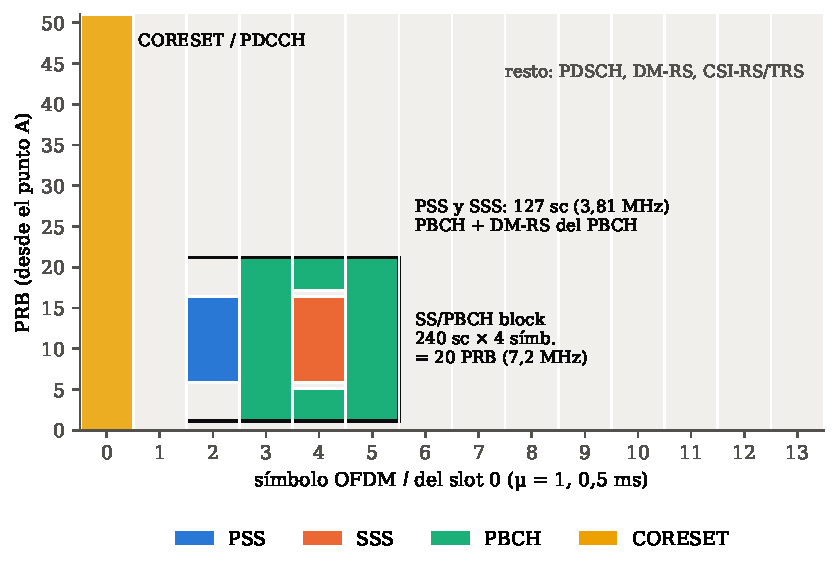
\includegraphics[width=0.85\linewidth]{figuras/fig_grilla_ssb.pdf}
\caption{Grilla tiempo-frecuencia del slot~0 de la celda n78 (51~PRB, 30~kHz). El SSB ocupa los símbolos 2 a 5 (caso~C, primer SSB de la ráfaga) y empieza 14 subportadoras por encima del punto A. El CORESET del primer símbolo es ilustrativo.}
\label{fig:grilla}
\end{figure}

La posición en el tiempo depende del ``caso'' de TS~38.213 §4.1. En n78, con 30~kHz, es el \textbf{caso~C}: los SSB empiezan en los símbolos $\{2,8\}+14n$ del medio de trama, y en esta banda hay hasta $L_\text{max}=8$ SSB por ráfaga, uno por haz posible. La celda transmite solo el primero (\texttt{ssb-PositionsInBurst} = \texttt{10000000}), porque tiene una sola antena y no hace barrido de haces: ocupa los símbolos 2 a 5 del slot~0. En n3, con 15~kHz, es el \textbf{caso~A}, con $L_\text{max}=4$.

\subsubsection{Identidad física de la celda (PCI)}\label{sec:pci}
NR tiene 1008 PCI, que se obtienen como \cite[§7.4.2.1]{ts38211}
\begin{equation}
N_\text{ID}^\text{cell} = 3N_\text{ID}^{(1)} + N_\text{ID}^{(2)}, \qquad N_\text{ID}^{(1)}\in\{0,\dots,335\},\ N_\text{ID}^{(2)}\in\{0,1,2\}.
\label{eq:pci}
\end{equation}
El PSS codifica $N_\text{ID}^{(2)}$ y el SSS codifica $N_\text{ID}^{(1)}$ (dependiendo también de $N_\text{ID}^{(2)}$). Para el PCI~1 de la celda:
\begin{equation}
1 = 3\cdot 0 + 1 \;\Rightarrow\; N_\text{ID}^{(1)} = 0,\quad N_\text{ID}^{(2)} = 1.
\end{equation}

\paragraph{PSS.} La secuencia del PSS es \cite[§7.4.2.2.1]{ts38211}
\begin{equation}
d_\text{PSS}(n) = 1 - 2x(m),\qquad m = \left(n + 43N_\text{ID}^{(2)}\right) \bmod 127,\qquad 0\le n<127,
\label{eq:pss}
\end{equation}
con $x(i+7) = \left(x(i+4)+x(i)\right)\bmod 2$ y estado inicial $[x(6)\dots x(0)] = [1\,1\,1\,0\,1\,1\,0]$. Es una \textbf{m-secuencia} de longitud $2^7-1 = 127$ en BPSK. Los tres PSS son la misma secuencia con desplazamientos cíclicos de 0, 43 y 86. Para la celda, $N_\text{ID}^{(2)}=1$ da un desplazamiento de 43.

\paragraph{SSS.} La secuencia del SSS es \cite[§7.4.2.3.1]{ts38211}
\begin{equation}
d_\text{SSS}(n) = \left[1-2x_0\big((n+m_0)\bmod 127\big)\right]\left[1-2x_1\big((n+m_1)\bmod 127\big)\right],
\label{eq:sss}
\end{equation}
\begin{equation}
m_0 = 15\left\lfloor \frac{N_\text{ID}^{(1)}}{112}\right\rfloor + 5N_\text{ID}^{(2)},\qquad m_1 = N_\text{ID}^{(1)} \bmod 112,
\end{equation}
donde $x_0$ y $x_1$ son dos m-secuencias de longitud 127 con polinomios distintos ($x_0(i+7)=(x_0(i+4)+x_0(i))\bmod 2$ y $x_1(i+7)=(x_1(i+1)+x_1(i))\bmod 2$). Para la celda, $m_0 = 0 + 5 = 5$ y $m_1 = 0$. El producto de dos m-secuencias desplazadas es una secuencia de tipo \textbf{Gold} (\cref{sec:secuencias}).

\paragraph{PBCH.} Lleva el bloque BCH de 24~bits (los 23 del MIB más el bit que identifica el tipo de mensaje BCCH-BCH) y 8~bits que agrega la capa física: los 4 bits menos significativos del SFN, el bit de medio de trama y, con $L_\text{max}=8$ como en esta celda, el bit más significativo de $k_\text{SSB}$ y dos bits reservados (los bits altos del índice del SSB solo se transmiten así cuando $L_\text{max}=64$, en FR2). Son 32~bits, que con el CRC de 24~bits forman 56~bits; se codifican con código polar ($N=512$), se adaptan a $E=864$~bits y se modulan en QPSK: 432 símbolos, que llenan las 576~RE del PBCH menos las 144 de su DM-RS \cite{ts38212}\verif. La DM-RS del PBCH ocupa una de cada cuatro subportadoras, con un desplazamiento $v = N_\text{ID}^\text{cell}\bmod 4$, que en esta celda vale 1. Su secuencia depende del índice del SSB, así que el UE averigua de qué SSB de la ráfaga se trata sin decodificar nada.

\subsection{MIB y SIB1}\label{sec:mib}
El \textbf{MIB} \cite[§6.2.2]{ts38331} contiene lo mínimo para encontrar el SIB1:
\begin{itemize}
  \item los 6 bits más significativos del SFN;
  \item \texttt{subCarrierSpacingCommon}: la SCS del SIB1 y de los mensajes iniciales;
  \item \texttt{ssb-SubcarrierOffset} ($k_\text{SSB}$);
  \item \texttt{dmrs-TypeA-Position}: si la primera DM-RS del PDSCH va en el símbolo 2 o en el 3;
  \item \texttt{pdcch-ConfigSIB1}: los índices \texttt{controlResourceSetZero} y \texttt{searchSpaceZero}, que fijan la ubicación del CORESET~0 y las ocasiones de monitoreo del PDCCH del SIB1;
  \item \texttt{cellBarred} e \texttt{intraFreqReselection}.
\end{itemize}

El \textbf{SIB1} se transmite en el PDSCH. En la celda n78 incluía, entre otros parámetros:
\begin{itemize}
  \item el PLMN y el TAC (7);
  \item \texttt{q-RxLevMin} = $-70$, en pasos de 2~dB, o sea, $-140$~dBm \verif;
  \item la portadora: 51~PRB a 30~kHz y \texttt{offsetToPointA} = 2;
  \item el patrón TDD de 5~ms (\cref{sec:tdd});
  \item la configuración del PRACH (\cref{sec:rach});
  \item \texttt{ss-PBCH-BlockPower} = $-16$~dBm, usado por el UE para estimar la pérdida de trayecto (\cref{sec:potencia_ul});
  \item el ciclo de paging por defecto, de 128 tramas (1,28~s);
  \item los temporizadores RRC T300, T310 y T311.
\end{itemize}

\subsection{Señales piloto: DM-RS, CSI-RS y TRS}\label{sec:pilotos}
LTE transmitía una señal de referencia común (CRS) en todas las subframes y en todo el ancho de banda, haya o no tráfico. NR la eliminó (\emph{lean carrier}) para reducir la interferencia y el consumo, y repartió sus funciones entre señales específicas, que solo se transmiten cuando hacen falta \cite[§7.4.1]{ts38211}:
\begin{itemize}
  \item \textbf{DM-RS} (\emph{demodulation reference signal}): va dentro de la asignación del PDSCH, del PDCCH y del PBCH, y permite estimar el canal para demodular coherentemente ese canal. En el PDSCH es \emph{front-loaded}: la primera DM-RS va al principio de la asignación, para que el receptor empiece a demodular cuanto antes. Puede haber posiciones adicionales, cuando el canal varía rápido (Doppler). En el PDCCH, ocupa las subportadoras 1, 5 y 9 de cada REG.
  \item \textbf{CSI-RS} (\emph{channel state information reference signal}): permite que el UE mida el canal y reporte el CSI (CQI, PMI, RI). El gNB usa el CQI para elegir el MCS. El reporte puede ser periódico (por PUCCH; en esta celda, formato~2) o aperiódico (por PUSCH, cuando lo pide un DCI).
  \item \textbf{TRS} (\emph{tracking reference signal}): es un conjunto de CSI-RS de un puerto, en dos slots consecutivos, que el UE usa para el seguimiento fino de tiempo y frecuencia \cite[§5.1.6.1.1]{ts38214}\verif. Cumple la función de sincronismo continuo que en LTE hacía la CRS.
  \item \textbf{PT-RS} (\emph{phase tracking}): corrige el ruido de fase. Se usa sobre todo en FR2.
\end{itemize}
Esta separación es coherente con una observación de la \cref{sec:crono}: al deshabilitar los CSI-RS para evitar las fallas de enlace por CSI, la celda también dejó de transmitir el TRS y el enlace empeoró. No se midió directamente si el UE dejó de corregir su deriva, pero es la explicación más probable.

\subsection{PDCCH y PDSCH}\label{sec:pdcch}
\paragraph{PDCCH.} Lleva el DCI, que contiene las asignaciones de bajada (formatos 1\_0 y 1\_1), los \emph{grants} de subida (0\_0 y 0\_1) y los comandos de potencia. Se transmite en un \textbf{CORESET}, una región de 1 a 3 símbolos y un múltiplo de 6~PRB. Su unidad es el REG (1~PRB $\times$ 1 símbolo); 6~REG forman un CCE, y un PDCCH ocupa 1, 2, 4, 8 o 16~CCE (nivel de agregación), según la robustez necesaria \cite[§7.3.2]{ts38211}. El DCI se codifica con código polar y siempre se modula en QPSK.

El UE no sabe a priori dónde está su PDCCH: lo busca a ciegas (\emph{blind decoding}) en un \textbf{espacio de búsqueda}, un conjunto de candidatos en CCE y niveles de agregación. El CRC del DCI va enmascarado con el RNTI del destinatario, y el UE se queda con el candidato cuyo CRC verifica con su RNTI. En el SIB1 de la celda, el espacio de búsqueda común~1 está en el CORESET~0 y en el primer símbolo del slot, con 2 candidatos de nivel de agregación~4, para los DCI 0\_0 y 1\_0.

\paragraph{PDSCH.} Lleva los datos de usuario, el SIB1, el paging y la RAR. Ocupa entre 2 y 14 símbolos del slot (mapeo tipo A o B), y el DCI fija su ubicación, el MCS y el proceso HARQ. Se transmite $k_0$ slots después del DCI y el UE confirma la recepción con un HARQ-ACK $k_1$ slots después \cite{ts38214}. En TDD, ese ACK tiene que esperar un slot de subida.

\subsection{Scrambling}\label{sec:scrambling}
Antes de modular, cada bloque de bits codificados $b(i)$ se aleatoriza con una secuencia pseudoaleatoria $c(i)$ \cite[§7.3.1.1]{ts38211}:
\begin{equation}
\tilde{b}(i) = \left(b(i) + c(i)\right)\bmod 2,
\label{eq:scr}
\end{equation}
donde $c(i)$ es la secuencia Gold de TS~38.211 §5.2.1 (\cref{sec:secuencias}). Su inicialización depende del canal:
\begin{align}
\text{PDSCH:}&\quad c_\text{init} = n_\text{RNTI}\cdot 2^{15} + q\cdot 2^{14} + n_\text{ID}, \label{eq:cinit_pdsch}\\
\text{PUSCH:}&\quad c_\text{init} = n_\text{RNTI}\cdot 2^{15} + n_\text{ID}, \label{eq:cinit_pusch}\\
\text{PDCCH:}&\quad c_\text{init} = \left(n_\text{RNTI}\cdot 2^{16} + n_\text{ID}\right)\bmod 2^{31},
\end{align}
donde $n_\text{ID}$ es el PCI (o un identificador configurado), $n_\text{RNTI}$ es el identificador del UE y $q$ es la palabra de código \cite[§6.3.1.1, §7.3.1.1, §7.3.2.3]{ts38211}.

\textbf{Por qué se hace el scrambling.}
\begin{enumerate}
  \item \textbf{Aleatorización de la interferencia entre celdas.} Dos celdas vecinas usan secuencias distintas, porque dependen del PCI. El receptor desaleatoriza con la secuencia de su celda: la señal útil queda intacta y la interferencia de la vecina queda multiplicada por una secuencia que no le corresponde, por lo que se comporta como ruido blanco. Sin scrambling, una interferencia con la misma estructura de bits podría correlacionarse con la señal útil y sesgar al decodificador.
  \item \textbf{Separación entre UE.} Como $c_\text{init}$ incluye el RNTI, una transmisión destinada a otro UE no decodifica bien después de la desaleatorización.
  \item \textbf{Balance y espectro.} Rompe las secuencias largas de ceros o unos y los patrones repetitivos: la constelación se usa de manera equiprobable, la potencia media es estable y el espectro no tiene líneas espectrales.
  \item \textbf{Información implícita.} En el PBCH, el scrambling también depende de bits del SFN y del índice del SSB. Así se puede combinar el PBCH de varias repeticiones.
\end{enumerate}

\subsection{Codificación de canal: LDPC y Polar}\label{sec:codificacion}
NR usa dos familias de códigos \cite{ts38212}:
\begin{itemize}
  \item \textbf{LDPC} para los datos (DL-SCH y UL-SCH). Son códigos cuasi-cíclicos definidos por dos matrices base: el \emph{base graph}~1 (BG1, bloques de hasta 8448~bits, tasa madre 1/3), para bloques grandes y tasas altas, y el BG2 (hasta 3840~bits, tasa madre 1/5), para bloques chicos y tasas bajas. Su estructura permite decodificar en paralelo con alto throughput y baja latencia, y admite HARQ con redundancia incremental: el transmisor lee un \emph{circular buffer} desde distintas versiones de redundancia (RV~0 a 3). El BG se elige con el tamaño del bloque y la tasa de código \cite[§7.2.2]{ts38212}\verif.
  \item \textbf{Polar} para el control: DCI, el BCH del PBCH y la UCI de más de 11~bits. Alcanzan la capacidad asintóticamente y, con decodificación por lista asistida por CRC (CA-SCL), funcionan muy bien con bloques cortos, que es el caso de la información de control. Las UCI de 3 a 11~bits usan Reed-Muller; las de 1 o 2~bits, repetición o simplex.
\end{itemize}
La segmentación en \emph{code blocks} se trata en la \cref{sec:cb}.

\subsection{Propiedades de las secuencias}\label{sec:secuencias}
La capa física de NR se apoya en tres familias de secuencias, que se eligen por sus propiedades de correlación y de envolvente.

\subsubsection{m-secuencias (PSS)}
Una m-secuencia es la salida de un registro de desplazamiento con realimentación lineal (LFSR) de $n$ etapas cuyo polinomio es primitivo. Sus propiedades son:
\begin{enumerate}
  \item \textbf{Período máximo:} $N = 2^n - 1$ (127 para $n=7$).
  \item \textbf{Balance:} cada período tiene $2^{n-1}$ unos y $2^{n-1}-1$ ceros: en BPSK, la media es casi nula.
  \item \textbf{Rachas:} la mitad de las rachas tiene longitud 1, un cuarto longitud 2, etc., como una secuencia aleatoria.
  \item \textbf{Autocorrelación periódica de dos valores:} con el mapeo $\pm 1$,
  \begin{equation}
  R(k) = \sum_{n=0}^{N-1} d(n)\,d\big((n+k)\bmod N\big) =
  \begin{cases} N & k\equiv 0 \pmod N\\ -1 & \text{en otro caso.}\end{cases}
  \label{eq:autocorr_m}
  \end{equation}
\end{enumerate}
La última propiedad hace que el pico de correlación sea nítido ($127$ contra $-1$) y que los tres PSS, que son desplazamientos cíclicos de la misma m-secuencia, estén casi ortogonales entre sí. LTE usaba secuencias Zadoff-Chu en el PSS. NR pasó a m-secuencias porque la correlación de una ZC con desvío de frecuencia presenta un pico desplazado en el tiempo (ambigüedad tiempo-frecuencia). En la búsqueda inicial, con un CFO todavía grande, eso produce errores de temporización. Las m-secuencias BPSK no tienen ese acoplamiento.

\subsubsection{Secuencias Gold (SSS y scrambling)}
Una secuencia Gold es la suma módulo~2 (en $\pm 1$, el producto) de dos m-secuencias de igual longitud que forman un \emph{par preferido}, con desplazamientos relativos distintos. Con $n$ etapas se obtienen $2^n+1$ secuencias, cuya correlación cruzada periódica toma solo tres valores, acotados en módulo por
\begin{equation}
t(n) = 1 + 2^{\lfloor (n+2)/2\rfloor}.
\end{equation}
Es decir, se sacrifica parte de la autocorrelación ideal de la m-secuencia a cambio de \textbf{una familia grande con correlación cruzada baja y acotada}. Eso es lo que hace falta para distinguir muchas identidades:
\begin{itemize}
  \item en el SSS, dos m-secuencias de 127 con desplazamientos $m_0$ y $m_1$ dan las 1008 combinaciones del PCI (\cref{eq:sss});
  \item en el scrambling, la secuencia de TS~38.211 §5.2.1 sale de un generador Gold con dos registros de 31 etapas (período nominal $2^{31}-1$), del que cada canal usa el segmento que necesita:
  \begin{equation}
  \begin{aligned}
  c(n) &= \left(x_1(n+N_C) + x_2(n+N_C)\right)\bmod 2,\\
  x_1(n+31) &= \left(x_1(n+3)+x_1(n)\right)\bmod 2,\\
  x_2(n+31) &= \left(x_2(n+3)+x_2(n+2)+x_2(n+1)+x_2(n)\right)\bmod 2,
  \end{aligned}
  \label{eq:gold}
  \end{equation}
  con $N_C = 1600$. $x_1$ se inicializa siempre igual, y $x_2$, con $c_\text{init}$. Los $2^{31}$ valores posibles de $c_\text{init}$ dan secuencias distintas para cada combinación de celda, RNTI y canal. Descartar las primeras 1600 muestras desacopla secuencias con valores de $c_\text{init}$ parecidos.
\end{itemize}

\subsubsection{Secuencias Zadoff-Chu (PRACH y secuencias de baja PAPR)}
La secuencia ZC de raíz $u$ y longitud $L$ impar es
\begin{equation}
x_u(n) = e^{-j\pi u n(n+1)/L},\qquad 0\le n < L,
\label{eq:zc}
\end{equation}
con $\gcd(u,L)=1$. Es la que usa el PRACH, con $L_\text{RA}=139$ en este caso \cite[§6.3.3.1]{ts38211}. Sus propiedades son:
\begin{enumerate}
  \item \textbf{Amplitud constante (CAZAC):} $|x_u(n)|=1$. Su DFT también es una ZC (escalada y conjugada), así que también tiene amplitud constante en frecuencia. Eso da una PAPR baja y una excitación pareja de todas las subportadoras, ideal para estimar el canal.
  \item \textbf{Autocorrelación periódica ideal:} es nula para todo desplazamiento cíclico distinto de cero. Los desplazamientos cíclicos de una misma raíz son, entonces, \textbf{ortogonales}, y sirven como preámbulos distintos si el desplazamiento supera el retardo máximo (\emph{zona de correlación cero}).
  \item \textbf{Correlación cruzada constante:} si $L$ es primo, la correlación cruzada periódica entre raíces distintas vale $\sqrt{L}$ en módulo para todo desplazamiento (normalizada, $1/\sqrt{L}$). Para $L=139$ es $\approx 0{,}085$, unos $-21$~dB.
\end{enumerate}
Las secuencias de la DM-RS del PUSCH con DFT-s-OFDM y las del PUCCH formatos 0 y 1 derivan de ZC (para longitudes $\ge 36$) o son secuencias QPSK buscadas por computadora con propiedades similares (longitudes menores) \cite[§5.2.2]{ts38211}.

\subsection{OFDMA y su PAPR: enfoque probabilístico}\label{sec:papr}
\subsubsection{La señal OFDM como suma de muchas subportadoras}
Un símbolo OFDM con $N$ subportadoras moduladas por símbolos $X_k$ independientes, de media nula y potencia unitaria, es
\begin{equation}
x(t) = \frac{1}{\sqrt{N}}\sum_{k=0}^{N-1} X_k\, e^{j2\pi k\Delta f t},\qquad 0\le t<T_u.
\label{eq:ofdm}
\end{equation}
La PAPR del símbolo es
\begin{equation}
\text{PAPR} = \frac{\max_{t}|x(t)|^2}{\mathrm{E}\{|x(t)|^2\}}.
\label{eq:papr}
\end{equation}
Para símbolos de módulo constante (por ejemplo, QPSK), el máximo absoluto es $N$ (todas las subportadoras en fase): 27,9~dB para $N=612$. Con QAM de amplitud variable y normalizando por la potencia media del conjunto, el máximo es mayor, porque también cuentan los puntos exteriores de la constelación. Pero esos valores exigen un patrón de datos particular, cuya probabilidad es despreciable. \textbf{La PAPR es una variable aleatoria}, y lo que importa es su distribución.

\subsubsection{Distribución}
Por el teorema central del límite, para $N$ grande cada muestra $x(t)$ es una suma de muchas variables independientes y se \emph{aproxima} a una gaussiana compleja de media nula. Lo que sigue es, entonces, una aproximación gaussiana, que mejora al crecer $N$; las muestras tampoco son exactamente independientes entre sí. Su envolvente tiene distribución de Rayleigh y su potencia instantánea normalizada, $|x|^2/\mathrm{E}\{|x|^2\}$, es exponencial de media~1:
\begin{equation}
\Pr\left\{\frac{|x(t)|^2}{\mathrm{E}\{|x|^2\}} > \gamma_0\right\} = e^{-\gamma_0}.
\end{equation}
Si se toman $N$ muestras independientes por símbolo (muestreo a Nyquist), la probabilidad de que \emph{ninguna} supere el umbral es $(1-e^{-\gamma_0})^N$, y la CCDF de la PAPR queda
\begin{equation}
\Pr\{\text{PAPR} > \gamma_0\} = 1 - \left(1 - e^{-\gamma_0}\right)^{N}.
\label{eq:ccdf}
\end{equation}
La señal analógica tiene picos entre muestras. Una aproximación empírica habitual es reemplazar $N$ por $\alpha N$, con $\alpha\approx 2{,}8$ \cite{vannee}.

\subsubsection{Por qué crece con \texorpdfstring{$N$}{N}: más probabilidad de picos}
Para umbrales altos, $e^{-\gamma_0}\ll 1$ y la \cref{eq:ccdf} se aproxima por
\begin{equation}
\Pr\{\text{PAPR} > \gamma_0\} \approx \alpha N\, e^{-\gamma_0}.
\label{eq:ccdf_aprox}
\end{equation}
\textbf{No es que todos los símbolos tengan más PAPR al aumentar $N$:} la potencia media y la distribución de cada muestra no cambian. Lo que crece es la cantidad de muestras ``candidatas'' por símbolo, y con ella la probabilidad de que alguna supere el umbral. Despejando el umbral que se supera con probabilidad $p$,
\begin{equation}
\gamma_0(p) \approx \ln\frac{\alpha N}{p},
\end{equation}
que crece solo \emph{logarítmicamente} con $N$. Por ejemplo, para $p=10^{-3}$, la aproximación da $10\log_{10}\ln(2{,}8\cdot 16/10^{-3}) = 10{,}3$~dB para $N=16$ y $10\log_{10}\ln(2{,}8\cdot 1024/10^{-3}) = 11{,}7$~dB para $N=1024$.

La \cref{fig:papr} (izquierda) muestra la CCDF, con la PAPR normalizada por la potencia media de cada símbolo, obtenida por simulación de Monte Carlo (20\,000 símbolos QPSK por curva, sobremuestreo $\times 4$). Al nivel $10^{-3}$, la PAPR pasa de 9,7~dB con $N=16$ a 10,7~dB con $N=64$, 11,4~dB con $N=256$ y 11,7~dB con $N=1024$. Es un aumento de la \emph{probabilidad} de picos altos que se ve como un desplazamiento lento de la curva hacia la derecha.

\begin{figure}[htbp]
\centering
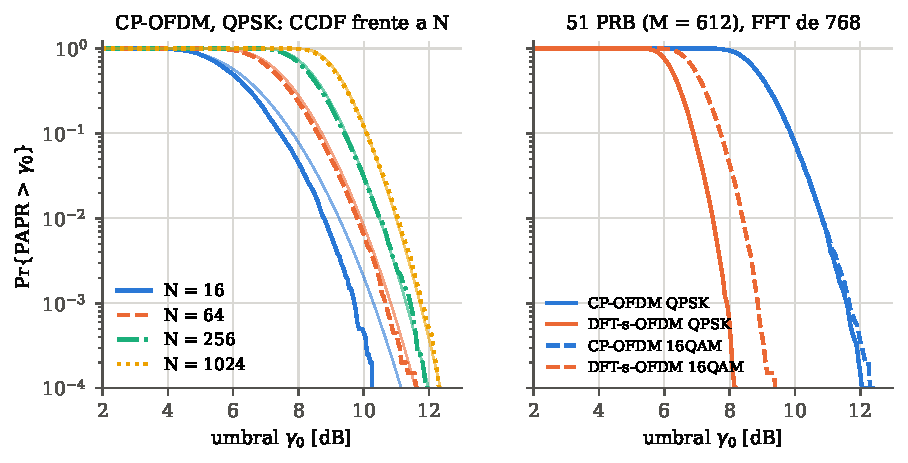
\includegraphics[width=\linewidth]{figuras/fig_ccdf_papr.pdf}
\caption{CCDF de la PAPR obtenida por simulación (Monte Carlo, 20\,000 símbolos por curva, sobremuestreo $\times 4$). Izquierda: CP-OFDM con QPSK para varios $N$; los trazos finos son la aproximación \eqref{eq:ccdf} con $\alpha=2{,}8$. Derecha: CP-OFDM contra DFT-s-OFDM con 612 subportadoras en una FFT de 768. Es una ilustración matemática con el mismo ancho para ambas formas de onda: 51~PRB no es una asignación válida de DFT-s-OFDM en NR (\cref{eq:235}), pero con 50~PRB el resultado es prácticamente el mismo.}
\label{fig:papr}
\end{figure}

\subsubsection{Consecuencia: el amplificador}
Un amplificador de potencia tiene que trabajar en su zona lineal para no distorsionar los picos. Si no, aparecen productos de intermodulación que ensucian la constelación (EVM) y emiten fuera de banda (ACLR). Para que la señal se mantenga lineal con probabilidad $1-p$, la potencia media tiene que quedar un \emph{back-off} de $\approx\gamma_0(p)$ por debajo de la saturación, y eso reduce la eficiencia del amplificador. En el gNB, alimentado por la red eléctrica, se acepta y se compensa con técnicas de reducción de crestas. En el UE, con batería y un amplificador barato, es una limitación seria: por eso NR ofrece DFT-s-OFDM en la subida (\cref{sec:dfts}).

En OFDMA, la señal con más subportadoras activas, \textbf{la del gNB en la bajada}, que suma las de todos los usuarios, es la que tiene estadísticamente la mayor PAPR. La de un UE en la subida con CP-OFDM tiene una PAPR algo menor si ocupa pocos PRB. Sin embargo, como la dependencia con $N$ es logarítmica, sigue estando muy por encima de la de DFT-s-OFDM.

\subsection{Presupuesto de potencia en el downlink}\label{sec:potencia_dl}
La magnitud que se especifica en la bajada es la \textbf{EPRE} (\emph{energy per resource element}): la potencia media por RE. Para dimensionar, se usa un modelo simplificado: carga completa, una potencia total $P_\text{tot}$ y una distribución uniforme sobre las $12N_\text{RB}$ subportadoras. Entonces,
\begin{equation}
\text{EPRE}~[\text{dBm}] = P_\text{tot}~[\text{dBm}] - 10\log_{10}(12\,N_\text{RB}).
\label{eq:epre}
\end{equation}
Para 51~PRB, $10\log_{10}(612) = 27{,}9$~dB, y para 106~PRB, $10\log_{10}(1272)=31{,}0$~dB. Es decir, en este modelo y con la misma potencia total, la EPRE de la celda n3 quedaría 3,1~dB por debajo de la de la n78. No se midió.

El presupuesto se asigna así:
\begin{itemize}
  \item \textbf{Densidad espectral aproximadamente constante.} La norma no define en la bajada un lazo cerrado de control de potencia por UE como el de la subida. El criterio habitual, y el de este análisis, es transmitir con una EPRE aproximadamente constante y adaptar la \emph{tasa} de cada UE (MCS) con el CQI que este reporta: un UE lejano no recibe más potencia, sino un MCS más robusto. Cómo reparte la potencia esta implementación no se relevó.
  \item \textbf{Relaciones entre señales.} La norma fija o señaliza relaciones de EPRE entre canales: el UE puede suponer que la EPRE del PSS y la del SSS difieren en 0 o 3~dB (\emph{boosting} del PSS) \cite[§4.1]{ts38213}; la del CSI-RS respecto del SSB se señaliza con \texttt{powerControlOffsetSS}; y la de la DM-RS del PDSCH respecto de los datos depende de cuántos grupos CDM quedan sin datos \cite[§4.1]{ts38214}\verif.
  \item \textbf{Referencia para la subida.} El gNB difunde la EPRE nominal del SSB (\texttt{ss-PBCH-BlockPower}, $-16$~dBm en esta celda) para que el UE estime la pérdida de trayecto como $PL = \texttt{ss-PBCH-BlockPower} - \text{RSRP}$, que entra en el control de potencia de la subida (\cref{sec:potencia_ul}).
\end{itemize}
Si todas las RE tuvieran la EPRE nominal del SSB, la potencia total nominal sería $-16 + 27{,}9 = 11{,}9$~dBm. En esta implementación ese valor es solo nominal: la potencia real radiada depende de la ganancia de transmisión de la B210 (80~dB configurados), de la frecuencia y de la antena, y no se calibró. Por lo tanto, la pérdida de trayecto que estima el UE está sesgada, y el lazo cerrado del control de potencia de la subida es el que corrige ese sesgo.

\section{Uplink y métodos de acceso}\label{sec:ul}

En la subida, muchos UE comparten un mismo recurso y ninguno conoce a priori el estado de los demás. NR resuelve el acceso con dos mecanismos complementarios:
\begin{itemize}
  \item el \textbf{acceso aleatorio con contienda} por el PRACH, para el primer contacto o cuando se pierde la sincronización;
  \item el \textbf{acceso planificado} (\emph{grant-based}), en el que el gNB asigna explícitamente los recursos del PUSCH.
\end{itemize}

\subsection{Acceso aleatorio por PRACH}\label{sec:rach}
\subsubsection{Configuración del PRACH de la celda}
El SIB1 de la celda n78 difunde la configuración de la \cref{tab:prach}, tomada del log del gNB (ver la nota de la \cref{sec:gscn}). El \texttt{prach-ConfigurationIndex}~159 de la tabla~6.3.3.2-3 de TS~38.211 (FR1, espectro no apareado) corresponde a:
\begin{itemize}
  \item formato \textbf{B4};
  \item $n_\text{SFN}\bmod x = y$ con $x=1$, $y=0$: una ocasión en \emph{todas} las tramas;
  \item subtrama~9, símbolo inicial~0, 1 slot de PRACH por subtrama, 1 ocasión por slot y una duración de 12 símbolos.
\end{itemize}
Con $\Delta f_\text{RA}=30$~kHz y un solo slot de PRACH por subtrama, la ocasión cae en el segundo slot de la subtrama~9, es decir, en el \textbf{slot~19} de la trama (\cref{fig:tdd}). Coincide con lo observado en los logs del gNB (\cref{sec:crono}).

\begin{table}[htbp]
\centering
\caption{Parámetros del PRACH difundidos en el SIB1 de la celda n78.}
\label{tab:prach}
\begin{tabular}{lll}
\toprule
Parámetro & Valor & Significado \\
\midrule
\texttt{prach-ConfigurationIndex} & 159 & B4, subtrama 9, cada 10~ms, 12 símbolos \\
\texttt{msg1-SubcarrierSpacing} & 30~kHz & $L_\text{RA}=139$, $\mu=1$ \\
\texttt{msg1-FrequencyStart} & 11 & primer PRB del PRACH \\
\texttt{msg1-FDM} & 1 & una ocasión en frecuencia \\
\texttt{prach-RootSequenceIndex} (\texttt{l139}) & 1 & primera raíz lógica \\
\texttt{zeroCorrelationZoneConfig} & 0 & $N_\text{CS}=0$ (tabla 6.3.3.1-7) \\
preámbulos por SSB & 64 & con contienda \\
\texttt{preambleReceivedTargetPower} & $-100$~dBm & potencia objetivo inicial \\
\texttt{powerRampingStep} & 4~dB & escalón de rampa \\
\texttt{preambleTransMax} & 7 & intentos máximos \\
\texttt{ra-ResponseWindow} & 20 slots & 10~ms para recibir la RAR \\
\texttt{ra-ContentionResolutionTimer} & 64 subtramas & 64~ms para el Msg4 \\
\bottomrule
\end{tabular}
\end{table}

Según la tabla~6.3.3.2-1 de TS~38.211, un preámbulo de $L_\text{RA}=139$ con $\Delta f_\text{RA}=\Delta f_\text{PUSCH}=30$~kHz ocupa 12~PRB: el PRACH de la celda ocupa los PRB~11 a~22, en el centro de la portadora.

\subsubsection{Preámbulos Zadoff-Chu}
Los preámbulos son secuencias ZC de longitud 139 (\cref{eq:zc}) y sus desplazamientos cíclicos \cite[§6.3.3.1]{ts38211}:
\begin{equation}
x_{u,v}(n) = x_u\big((n + C_v)\bmod L_\text{RA}\big),\qquad C_v = v\,N_\text{CS}.
\end{equation}
Cada raíz $u$ da $\lfloor L_\text{RA}/N_\text{CS}\rfloor$ preámbulos ortogonales, siempre que el desplazamiento $N_\text{CS}$ supere el retardo de ida y vuelta más el delay spread. Si no alcanza, se toman raíces consecutivas hasta completar los 64. En esta celda $N_\text{CS}=0$ y cada raíz aporta \textbf{un único} preámbulo ($C_0=0$): los 64 preámbulos salen de 64 raíces distintas, a partir del índice lógico~1.

Esta configuración tiene dos consecuencias. Por un lado, no hay zona de correlación cero que limitar: el pico de correlación puede estar en cualquier lugar del período, y el radio de la celda no lo limita la secuencia (\cref{sec:ta}). Por otro lado, los preámbulos ya no son ortogonales entre sí, sino que tienen la correlación cruzada constante de $1/\sqrt{139}\approx -21$~dB entre raíces. En una celda con un puñado de UE, esto no es un problema.

\subsubsection{Formato B4: duración, CP y tiempo de guarda}
Para el formato B4 con $\mu=1$ y $\kappa=64$ \cite[tabla~6.3.3.1-2]{ts38211}:
\begin{align}
N_u &= 12\cdot 2048\,\kappa\, 2^{-\mu} = 786\,432\,T_c = 400{,}0~\mu\text{s},\\
N_\text{CP}^\text{RA} &= 936\,\kappa\, 2^{-\mu} = 29\,952\,T_c = 15{,}23~\mu\text{s}.
\end{align}
Como la ocasión empieza justo en el instante de 0,5~ms de la subtrama, TS~38.211 §5.3.2 le suma $16\kappa = 1024\,T_c$ al CP: $N_\text{CP}^\text{RA} = 30\,976\,T_c = 15{,}76~\mu$s, y el preámbulo dura $817\,408\,T_c = 415{,}8~\mu$s. Los 12 símbolos del slot que reserva la ocasión (el primero, con CP largo) duran
\begin{equation}
(65\,536 + 5632) + 11\cdot(65\,536 + 4608) = 842\,752\,T_c = 428{,}6~\mu\text{s}.
\end{equation}
La diferencia es un \textbf{tiempo de guarda implícito} de $842\,752 - 817\,408 = 25\,344\,T_c = 12{,}9~\mu$s.

\subsubsection{Procedimiento de 4 pasos}
El procedimiento con contienda (\cref{fig:rach}) se define en TS~38.321 §5.1 y TS~38.213 §8:
\begin{enumerate}
  \item \textbf{Msg1 (preámbulo).} El UE elige al azar uno de los 64 preámbulos y lo transmite en la próxima ocasión de PRACH asociada al SSB que mejor recibe. Todavía no tiene timing advance: transmite con $N_\text{TA}=0$.
  \item \textbf{Msg2 (RAR).} El gNB detecta el preámbulo, mide su retardo y responde por PDSCH, planificado con un PDCCH enmascarado con el RA-RNTI. El RA-RNTI identifica la ocasión en la que se envió el preámbulo \cite[§5.1.3]{ts38321}:
  \begin{equation}
  \text{RA-RNTI} = 1 + s_\text{id} + 14\,t_\text{id} + 14\cdot 80\,f_\text{id} + 14\cdot 80\cdot 8\,\text{ul\_carrier\_id}.
  \end{equation}
  En la celda, $s_\text{id}=0$, $t_\text{id}=19$, $f_\text{id}=0$ y el portador UL es el normal (0): $\text{RA-RNTI} = 1 + 14\cdot 19 = 267$. La RAR lleva el identificador del preámbulo detectado, el comando de TA, un \emph{grant} para el Msg3 y un identificador temporal (TC-RNTI). El UE la espera durante la \texttt{ra-ResponseWindow} (10~ms).
  \item \textbf{Msg3.} El UE aplica el TA y transmite en el PUSCH asignado un \texttt{RRCSetupRequest} con su identidad (parte del 5G-S-TMSI o un número aleatorio de 39~bits).
  \item \textbf{Msg4 (resolución de contienda).} El gNB responde con un \texttt{RRCSetup} y un MAC~CE \emph{UE Contention Resolution Identity}, que repite los primeros 48~bits del Msg3 recibido. El UE que reconoce su propio Msg3 ganó la contienda y convierte el TC-RNTI en su C-RNTI. Los demás vuelven a empezar.
\end{enumerate}

\begin{figure}[htbp]
\centering
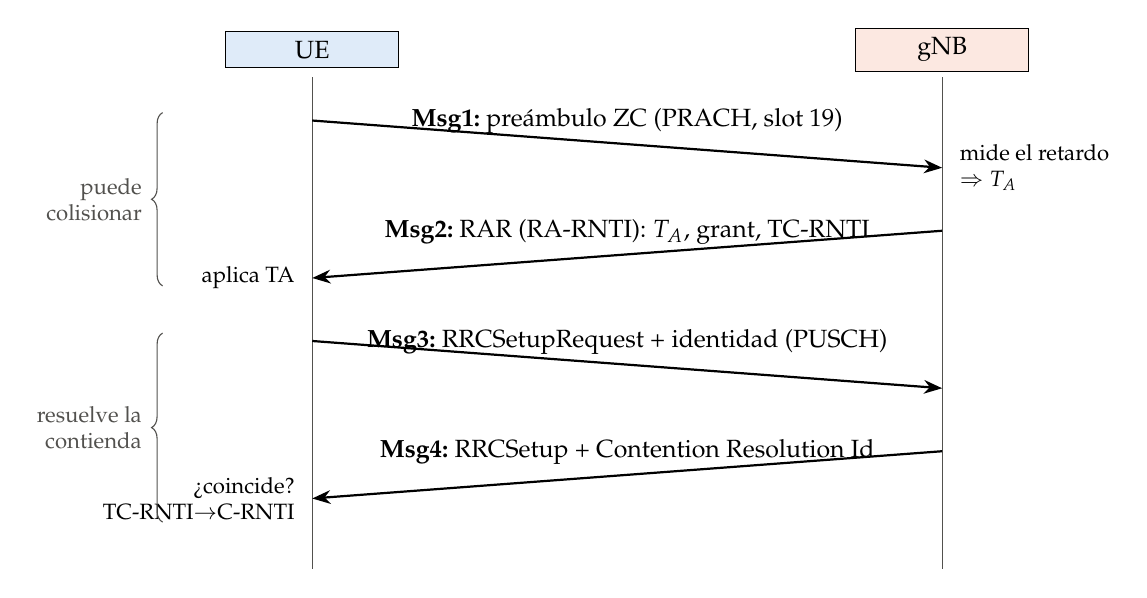
\begin{tikzpicture}[font=\small,>=Stealth]
  \node[draw,fill=azul!15,minimum width=2.2cm] (ue) at (0,0) {UE};
  \node[draw,fill=naranja!15,minimum width=2.2cm] (gnb) at (8,0) {gNB};
  \draw[gris] (0,-0.35) -- (0,-6.6);
  \draw[gris] (8,-0.35) -- (8,-6.6);
  \draw[->,thick] (0,-0.9) -- node[above,midway]{\textbf{Msg1:} preámbulo ZC (PRACH, slot 19)} (8,-1.5);
  \node[right,align=left,font=\footnotesize] at (8.1,-1.5) {mide el retardo\\$\Rightarrow T_A$};
  \draw[->,thick] (8,-2.3) -- node[above,midway]{\textbf{Msg2:} RAR (RA-RNTI): $T_A$, grant, TC-RNTI} (0,-2.9);
  \node[left,align=right,font=\footnotesize] at (-0.1,-2.9) {aplica TA};
  \draw[->,thick] (0,-3.7) -- node[above,midway]{\textbf{Msg3:} RRCSetupRequest + identidad (PUSCH)} (8,-4.3);
  \draw[->,thick] (8,-5.1) -- node[above,midway]{\textbf{Msg4:} RRCSetup + Contention Resolution Id} (0,-5.7);
  \node[left,align=right,font=\footnotesize] at (-0.1,-5.7) {¿coincide?\\TC-RNTI$\to$C-RNTI};
  \draw[decorate,decoration={brace,amplitude=4pt,mirror},gris] (-1.9,-0.8) -- (-1.9,-3.0) node[midway,left=4pt,align=right,font=\footnotesize]{puede\\colisionar};
  \draw[decorate,decoration={brace,amplitude=4pt,mirror},gris] (-1.9,-3.6) -- (-1.9,-6.0) node[midway,left=4pt,align=right,font=\footnotesize]{resuelve la\\contienda};
\end{tikzpicture}
\caption{Procedimiento de acceso aleatorio de 4 pasos con contienda (TS~38.321 §5.1; TS~38.213 §8).}
\label{fig:rach}
\end{figure}

\subsubsection{Analogía con ALOHA ranurado}
El PRACH es un canal de acceso múltiple aleatorio, y su análisis es el de \textbf{ALOHA ranurado}:
\begin{itemize}
  \item las \textbf{ranuras} son las ocasiones de PRACH (en esta celda, una cada 10~ms, es decir, 100 por segundo);
  \item dentro de cada ranura hay 64 ``subcanales'' ortogonales o casi ortogonales: los preámbulos;
  \item una \textbf{colisión} ocurre cuando dos o más UE eligen el mismo preámbulo en la misma ocasión.
\end{itemize}
Para ALOHA ranurado con llegadas de Poisson y carga $G$ intentos por ranura, la probabilidad de éxito de un intento es $e^{-G}$ y el throughput, $S = Ge^{-G}$, con un máximo de $1/e\approx 0{,}368$ en $G=1$. Para ALOHA puro, $S = Ge^{-2G}$ (máximo $1/(2e)$), porque el período vulnerable es el doble \cite{tanenbaum}. En el PRACH, la carga se reparte entre 64 preámbulos: si $k$ UE acceden en la misma ocasión, la probabilidad de que un UE dado no colisione es
\begin{equation}
\Pr\{\text{sin colisión}\} = \left(1 - \frac{1}{64}\right)^{k-1},
\label{eq:colision}
\end{equation}
que vale 0,98 para $k=2$ y 0,54 para $k=40$ (\cref{fig:aloha}).

\begin{figure}[htbp]
\centering
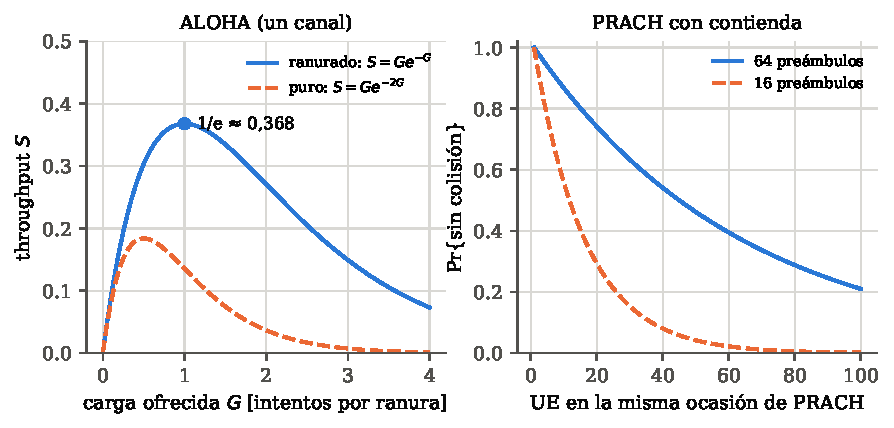
\includegraphics[width=\linewidth]{figuras/fig_aloha.pdf}
\caption{Izquierda: throughput de ALOHA ranurado y puro. Derecha: probabilidad de que un UE no colisione en una ocasión de PRACH, según la cantidad de UE que acceden en ella, con 64 y 16 preámbulos (\cref{eq:colision}).}
\label{fig:aloha}
\end{figure}

La diferencia con el ALOHA clásico está en \textbf{cómo se detecta y resuelve la colisión}. Dos UE que eligen el mismo preámbulo son indistinguibles para el gNB, que ve un solo pico de correlación (o dos picos cercanos) y responde con una sola RAR. Los dos UE creen haber sido escuchados y transmiten su Msg3 en el mismo grant: ahí sí colisionan. A lo sumo uno se decodifica (efecto captura) y el Msg4 lo identifica. El otro detecta que perdió al vencer el \texttt{ra-ContentionResolutionTimer} o al no reconocer su identidad, y reintenta tras un \emph{backoff} aleatorio, como en ALOHA. El costo de una colisión es, entonces, el tiempo de los cuatro mensajes, no solo una ranura.

\subsubsection{Power ramping}
El UE no conoce de antemano la potencia necesaria y la estima en lazo abierto \cite[§7.4]{ts38213}:
\begin{equation}
P_\text{PRACH} = \min\left\{P_\text{CMAX},\; P_\text{PRACH,target} + PL\right\}~[\text{dBm}],
\label{eq:pprach}
\end{equation}
donde $PL$ es la pérdida de trayecto estimada con el SSB, y la potencia objetivo, fijada por la MAC, crece en cada reintento \cite[§5.1.3]{ts38321}:
\begin{equation}
P_\text{PRACH,target} = \texttt{preambleReceivedTargetPower} + \Delta_\text{PREAMBLE} + (n-1)\cdot\texttt{powerRampingStep}.
\label{eq:ramping}
\end{equation}
Para el formato B4, $\Delta_\text{PREAMBLE} = 3\mu = 3$~dB \cite[tabla~7.3-2]{ts38321}. En la celda, el primer intento apunta a $-100 + 3 = -97$~dBm en el receptor del gNB, y el séptimo y último, a $-97 + 6\cdot 4 = -73$~dBm. Si se agota \texttt{preambleTransMax} sin RAR, la MAC informa un problema de acceso aleatorio a RRC. El escalonamiento evita que todos los UE transmitan con la máxima potencia, lo que aumentaría la interferencia y el consumo. Cada UE se acerca desde abajo a la potencia justa.

\subsubsection{Timing advance y radio de cobertura}\label{sec:ta}
Como la señal tarda $d/c$ en llegar al UE y otro tanto en volver, un UE a distancia $d$ que transmitiera alineado con la bajada que recibe llegaría al gNB con un retraso de $2d/c$. Para que las transmisiones de todos los UE lleguen alineadas a la grilla del gNB (y se conserve la ortogonalidad entre ellos), cada UE adelanta su trama de subida en \cite[§4.3.1]{ts38211}
\begin{equation}
T_\text{TA} = (N_\text{TA} + N_\text{TA,offset})\,T_c.
\label{eq:tta}
\end{equation}
$N_\text{TA,offset}$ es un adelanto fijo que deja tiempo de conmutación al gNB. En FR1 sin coexistencia LTE-NR vale $25\,600\,T_c\approx 13~\mu$s, y es el valor por defecto en FR1 cuando la red no señaliza \texttt{n-TimingAdvanceOffset} \cite[§7.1.2, tabla~7.1.2-2]{ts38133}. $N_\text{TA}$ compensa la ida y vuelta:
\begin{equation}
N_\text{TA}\,T_c = \frac{2d}{c}\quad\Longrightarrow\quad d = \frac{c\,N_\text{TA}\,T_c}{2}.
\label{eq:ta_d}
\end{equation}

\paragraph{Paso del TA.} Para una SCS de $2^\mu\cdot 15$~kHz, el comando de TA se expresa en múltiplos de $16\cdot 64\,T_c/2^\mu$ \cite[§4.2]{ts38213}. Con $\mu=1$:
\begin{equation}
\Delta T_\text{TA} = \frac{16\cdot 64}{2}\,T_c = 512\,T_c = 0{,}260~\mu\text{s}
\;\Rightarrow\;
\Delta d = \frac{c\,\Delta T_\text{TA}}{2} = \frac{3\cdot 10^8\cdot 0{,}260\cdot 10^{-6}}{2} \approx 39~\text{m}.
\end{equation}
\begin{itemize}
  \item \textbf{En la RAR}, el TA es absoluto: $T_A\in\{0,\dots,3846\}$ y $N_\text{TA} = T_A\cdot 16\cdot 64/2^\mu$ \cite[§4.2]{ts38213}. El máximo es $3846\cdot 0{,}260~\mu\text{s} = 1{,}0016$~ms, que corresponde a $d_\text{max}\approx 150$~km.
  \item \textbf{En la conexión}, el MAC~CE \emph{Timing Advance Command} es relativo: $N_\text{TA,new} = N_\text{TA,old} + (T_A-31)\cdot 16\cdot 64/2^\mu$, con $T_A\in\{0,\dots,63\}$, es decir, correcciones de $-31$ a $+32$ pasos.
\end{itemize}

\paragraph{El alcance geométrico lo limita el PRACH, no el TA.} Los 150~km que admite el campo de la RAR son una cota de señalización. La limitación física aparece \emph{antes} de que exista un TA: el preámbulo se transmite con $N_\text{TA}=0$ y llega al gNB con un retraso $2d/c$. Para que se lo pueda detectar sin interferir con lo que sigue tienen que cumplirse dos condiciones:
\begin{enumerate}
  \item el retardo más el delay spread tiene que caber en el CP del preámbulo, para que la ventana de correlación del gNB contenga un período completo de la secuencia: $2d/c + \tau_\text{max} \le T_\text{CP}^\text{RA}$;
  \item el preámbulo retrasado no tiene que invadir los símbolos siguientes: $2d/c \le T_\text{GT}$.
\end{enumerate}
Para el formato B4 con $\mu=1$:
\begin{align}
\text{por el CP:}\quad & d \le \frac{c\,T_\text{CP}^\text{RA}}{2} = \frac{3\cdot 10^8\cdot 15{,}76\cdot 10^{-6}}{2} \approx 2{,}36~\text{km}\quad(\tau_\text{max}=0),\\
\text{por la guarda:}\quad & d \le \frac{c\,T_\text{GT}}{2} = \frac{3\cdot 10^8\cdot 12{,}9\cdot 10^{-6}}{2} \approx 1{,}9~\text{km}.
\end{align}
El alcance geométrico de la configuración es, entonces, del orden de \textbf{2~km}. Es una cota temporal orientativa, calculada por el grupo sobre los valores de la norma, que no incluye el presupuesto de enlace, la sensibilidad ni la interferencia (el alcance radioeléctrico no se midió): si los símbolos 12 y 13 del slot~19 no se usan para otras transmisiones de subida, la guarda real es mayor y manda el límite del CP. Por eso los formatos largos ($L_\text{RA}=839$, con CP de hasta $\approx 684~\mu$s en el formato~1) se reservan para celdas de decenas de kilómetros, y los cortos, como el B4, para celdas chicas. En la jaula de Faraday, con distancias de metros, el TA inicial es prácticamente 0: lo que importa es su \emph{evolución} (\cref{sec:crono}).

Una vez conectado, el gNB mide continuamente el retardo de las señales de subida (DM-RS, SRS, PUCCH) y envía correcciones relativas. El CP de los símbolos de datos (2,34~$\mu$s) solo tiene que absorber el delay spread y el error residual de TA. El TA \emph{no} lo cubre.

\subsection{Acceso planificado (grant-based)}\label{sec:grant}
Una vez conectado, el UE no transmite datos cuando quiere. El gNB es el que asigna cada PUSCH:
\begin{enumerate}
  \item \textbf{Scheduling Request (SR).} Cuando llegan datos al buffer y el UE no tiene grant, envía un SR por el PUCCH, un pedido de un bit en recursos periódicos dedicados \cite[§5.4.4]{ts38321}, \cite[§9.2.4]{ts38213}.
  \item \textbf{Grant inicial.} El gNB responde con un DCI~0\_0 o 0\_1 en el PDCCH, que asigna PRB, MCS, proceso HARQ y el desfase $k_2$ entre el DCI y el PUSCH \cite[§6.1.2.1]{ts38214}. En el SIB1 de la celda, la tabla de asignación temporal común del PUSCH tiene $k_2\in\{4,5,6,7,11\}$ slots.
  \item \textbf{Buffer Status Report (BSR).} En ese primer PUSCH, el UE incluye un MAC~CE BSR con la cantidad de datos pendientes por grupo de canales lógicos \cite[§5.4.5]{ts38321}. Con esa información, el gNB dimensiona los grants siguientes.
  \item \textbf{Transmisión y HARQ.} El gNB decodifica cada PUSCH y, si falla, pide una retransmisión con otro DCI (HARQ asíncrono, hasta 16 procesos).
\end{enumerate}
El ciclo SR $\to$ grant $\to$ PUSCH le agrega latencia a la subida. En TDD, el SR solo se puede enviar en un slot de subida, el grant llega en uno de bajada, y el PUSCH vuelve a necesitar un slot de subida al menos $k_2\ge 4$ slots después. Esta es una de las causas de la asimetría y la latencia medidas (\cref{sec:resultados}).

Para reducir esa latencia, NR prevé el \textbf{configured grant} \cite[§5.8.2]{ts38321}: recursos de PUSCH periódicos preasignados que el UE usa sin pedirlos. El de tipo~1 se configura completo por RRC; el de tipo~2 se configura por RRC y se activa o desactiva con un DCI. Es la base de URLLC. En esta celda no se usó.

\subsection{Qué pasa cuando el celular está callado}\label{sec:callado}
Mantener al UE escuchando el PDCCH en todos los slots consume batería. NR escalona los estados según la actividad:
\begin{itemize}
  \item \textbf{DRX en RRC\_CONNECTED} \cite[§5.7]{ts38321}: el UE monitorea el PDCCH solo durante el \emph{on duration} de cada ciclo DRX (corto o largo). Cada vez que recibe un DCI con datos nuevos, arranca el \texttt{drx-InactivityTimer} y se queda despierto mientras haya actividad. Al vencer, vuelve al ciclo. El costo es latencia: un paquete que llega mientras el UE duerme espera al siguiente \emph{on duration}.
  \item \textbf{Paso a RRC\_INACTIVE o RRC\_IDLE} \cite[§4.2.1]{ts38331}: después de un período sin tráfico (temporizador de inactividad del gNB), la red libera la conexión con un \texttt{RRCRelease}. En RRC\_INACTIVE, el UE y la red guardan el contexto (seguridad, configuración) y la reanudación es rápida (\texttt{RRCResumeRequest}). En RRC\_IDLE se pierde el contexto de acceso radio y hay que volver a establecer la conexión.
  \item \textbf{Paging} \cite{ts38304}: en INACTIVE o IDLE, el UE se despierta solo en su \emph{paging occasion}, una vez por ciclo de paging (en la celda, 128 tramas = 1,28~s). Si la red tiene datos para él, lo llama por el PDCCH con el P-RNTI, y el UE inicia el acceso aleatorio.
  \item \textbf{Vencimiento del temporizador de TA} \cite[§5.2]{ts38321}: el TA que mantiene el gNB solo es válido mientras el UE se mueve poco. Si no recibe comandos de TA durante \texttt{timeAlignmentTimer}, el UE considera que perdió el sincronismo de subida: vacía los buffers HARQ, libera el PUCCH, el SRS y los configured grants, y \textbf{para volver a transmitir tiene que pasar otra vez por el RACH}. En la celda, \texttt{timeAlignmentTimerCommon} = \texttt{infinity} en el SIB1.
\end{itemize}

\subsection{CP-OFDM contra DFT-s-OFDM}\label{sec:dfts}
\subsubsection{Las dos formas de onda de la subida}
En la bajada, NR usa siempre CP-OFDM. En la subida admite dos formas de onda: CP-OFDM (sin precodificación por transformada) y \textbf{DFT-s-OFDM}, que se activa con \texttt{transformPrecoder} \cite[§6.3.1.4]{ts38211}. DFT-s-OFDM (equivalente al SC-FDMA de LTE) antepone a la IFFT una DFT de $M$ puntos sobre los símbolos de modulación de cada símbolo OFDM:
\begin{equation}
y(l\,M_\text{sc}^\text{PUSCH} + k) = \frac{1}{\sqrt{M_\text{sc}^\text{PUSCH}}}\sum_{i=0}^{M_\text{sc}^\text{PUSCH}-1} \tilde{x}(l\,M_\text{sc}^\text{PUSCH}+i)\,e^{-j\frac{2\pi i k}{M_\text{sc}^\text{PUSCH}}},
\label{eq:transform}
\end{equation}
con la restricción \cite[§6.3.1.4]{ts38211}
\begin{equation}
M_\text{sc}^\text{PUSCH} = 12\cdot 2^{\alpha_2}\cdot 3^{\alpha_3}\cdot 5^{\alpha_5},
\label{eq:235}
\end{equation}
que asegura que la DFT tenga solo factores primos chicos y se pueda calcular eficientemente. Hay una consecuencia práctica: \textbf{51~PRB no está permitido} ($51 = 3\cdot 17$), así que con DFT-s-OFDM el gNB asignó como máximo 50~PRB ($50 = 2\cdot 5^2$). Así se observó en la prueba A/B/A (\cref{sec:crono}). La transformación solo se admite con una capa.

\begin{figure}[htbp]
\centering
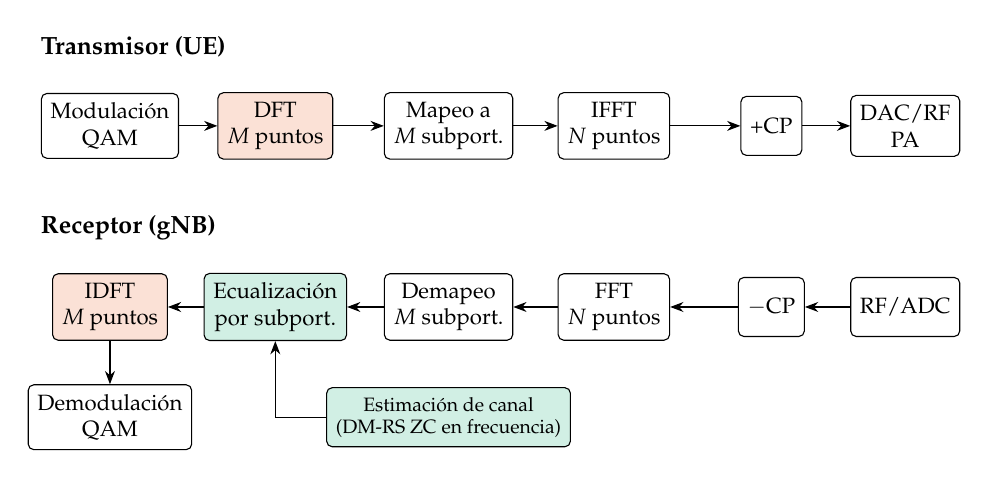
\begin{tikzpicture}[font=\footnotesize,>=Stealth,
  b/.style={draw,rounded corners=2pt,minimum height=0.75cm,align=center,fill=white},
  dft/.style={b,fill=naranja!20},
  eq/.style={b,fill=verde!20}]
  % Transmisor
  \node[font=\small\bfseries,anchor=west] at (-0.4,1.0) {Transmisor (UE)};
  \node[b] (mod) at (0.6,0) {Modulación\\QAM};
  \node[dft] (dftb) at (2.7,0) {DFT\\$M$ puntos};
  \node[b] (map) at (4.9,0) {Mapeo a\\$M$ subport.};
  \node[b] (ifft) at (7.0,0) {IFFT\\$N$ puntos};
  \node[b] (cp) at (9.0,0) {+CP};
  \node[b] (rf) at (10.7,0) {DAC/RF\\PA};
  \draw[->] (mod) -- (dftb); \draw[->] (dftb) -- (map); \draw[->] (map) -- (ifft); \draw[->] (ifft) -- (cp); \draw[->] (cp) -- (rf);
  % Receptor
  \node[font=\small\bfseries,anchor=west] at (-0.4,-1.3) {Receptor (gNB)};
  \node[b] (rrf) at (10.7,-2.3) {RF/ADC};
  \node[b] (rcp) at (9.0,-2.3) {$-$CP};
  \node[b] (fft) at (7.0,-2.3) {FFT\\$N$ puntos};
  \node[b] (dem) at (4.9,-2.3) {Demapeo\\$M$ subport.};
  \node[eq] (equ) at (2.7,-2.3) {Ecualización\\por subport.};
  \node[dft] (idft) at (0.6,-2.3) {IDFT\\$M$ puntos};
  \node[b] (det) at (0.6,-3.7) {Demodulación\\QAM};
  \draw[->] (rrf) -- (rcp); \draw[->] (rcp) -- (fft); \draw[->] (fft) -- (dem); \draw[->] (dem) -- (equ); \draw[->] (equ) -- (idft); \draw[->] (idft) -- (det);
  \node[eq,font=\scriptsize] (ce) at (4.9,-3.7) {Estimación de canal\\(DM-RS ZC en frecuencia)};
  \draw[->] (ce) -| (equ);
\end{tikzpicture}
\caption{Cadenas de DFT-s-OFDM. Los bloques naranjas (DFT/IDFT de $M$ puntos) son los que la diferencian de CP-OFDM: sin ellos, la cadena es la de CP-OFDM, y el ecualizador entrega directamente símbolos QAM. En verde, la ecualización en frecuencia, que va después de la FFT y del demapeo, y antes de la IDFT.}
\label{fig:dfts}
\end{figure}

\subsubsection{Por qué baja la PAPR}
Con mapeo localizado (subportadoras contiguas), la cadena DFT~$M$ $\to$ IFFT~$N$ equivale a interpolar los $M$ símbolos de modulación con un núcleo tipo sinc periódica. La señal en el tiempo es, en esencia, \textbf{una portadora única} que recorre los símbolos de la constelación uno tras otro. Su envolvente sigue, en los instantes de los símbolos, a la constelación (QPSK tiene allí amplitud constante); entre ellos, la interpolación genera picos moderados. La PAPR depende sobre todo de la modulación y mucho menos de $M$ que en CP-OFDM, donde cada muestra es la suma aproximadamente gaussiana de la \cref{sec:papr}.

La simulación ilustrativa de la \cref{fig:papr} (derecha), con 612 subportadoras en una FFT de 768, da al nivel $10^{-3}$:
\begin{itemize}
  \item CP-OFDM: $\approx 11{,}6$~dB, prácticamente igual con QPSK, 16QAM o 256QAM;
  \item DFT-s-OFDM: 7,9~dB con QPSK, 8,9~dB con 16QAM y 9,2~dB con 256QAM.
\end{itemize}
En esa simulación, la ventaja es de 2,5 a 3,7~dB, mayor cuanto más simple es la modulación. No es una medición del teléfono. Para el UE eso significa un back-off menor: con el mismo amplificador puede transmitir más potencia media (la norma le permite una reducción de potencia máxima, MPR, menor con DFT-s-OFDM: con QPSK, hasta 1~dB contra hasta 3~dB de CP-OFDM en las asignaciones de borde y externas \cite[§6.2.2, tabla~6.2.2-1]{ts38101}), o la misma potencia con más eficiencia.

\subsubsection{Cuándo conviene cada una}
\begin{itemize}
  \item \textbf{DFT-s-OFDM:} conviene cuando el UE está \textbf{limitado en potencia}, en el borde de la celda, donde el amplificador ya trabaja cerca de saturación y cada dB de back-off se traduce en alcance o en SINR. En ese régimen se usan modulaciones bajas (incluida $\pi/2$-BPSK, que solo existe con transform precoding), justo donde la ventaja de PAPR es mayor.
  \item \textbf{CP-OFDM:} conviene con \textbf{SINR alta} y potencia sobrante. Admite MIMO de varias capas, asignaciones de PRB no contiguas y cualquier cantidad de PRB, y cada subportadora conserva su propia SINR después de ecualizar. En canales selectivos en frecuencia y con MCS altos, suele rendir más.
\end{itemize}
Por eso el gNB puede cambiar de forma de onda según las condiciones del UE (la conmutación dinámica llegó en releases posteriores). En la prueba de la \cref{sec:crono}, con una SINR media de $\approx 27$~dB y el UE muy cerca de la antena, DFT-s-OFDM no mejoró el throughput, lo que es coherente con este análisis si el UE no estaba limitado en potencia.

\subsubsection{Dónde se ecualiza en DFT-s-OFDM}\label{sec:ecualizacion}
En el receptor (\cref{fig:dfts}), la ecualización se hace \textbf{en frecuencia, después de la FFT de $N$ puntos y del demapeo de las $M$ subportadoras, y antes de la IDFT de $M$ puntos} que deshace la precodificación. La justificación es la siguiente:
\begin{enumerate}
  \item Gracias al CP, después de la FFT el canal es \textbf{diagonal en frecuencia}: en cada subportadora, $R_k = H_k Y_k + W_k$. Un ecualizador de un coeficiente por subportadora (ZF $1/H_k$, o MMSE $H_k^*/(|H_k|^2+\sigma^2)$) invierte el canal con complejidad mínima, igual que en CP-OFDM. La DM-RS del PUSCH con DFT-s-OFDM se mapea directamente en frecuencia (una secuencia ZC de baja PAPR, sin precodificar), así que da $H_k$ en el mismo dominio.
  \item Después de la IDFT, cada muestra es una combinación de \emph{todas} las subportadoras, cada una afectada por un $H_k$ distinto: el canal deja de ser diagonal y aparece interferencia entre símbolos. Ecualizar ahí exigiría un ecualizador en el tiempo de muchos coeficientes, que es justamente lo que el CP permite evitar.
  \item La IDFT reparte el error residual y el ruido de forma pareja entre los $M$ símbolos, así que un desvanecimiento profundo en algunas subportadoras degrada un poco a todos los símbolos en lugar de borrar algunos. Es un promediado en frecuencia: el MMSE da una SINR efectiva única para toda la asignación. En CP-OFDM también se usa un único MCS por asignación, pero el decodificador LDPC recibe la confiabilidad propia de cada subportadora; en DFT-s-OFDM, el ruido realzado de las subportadoras débiles se reparte entre todos los símbolos. Por eso, en canales muy selectivos y con MCS altos, DFT-s-OFDM suele rendir algo menos.
\end{enumerate}
En CP-OFDM no hay IDFT de $M$ puntos: el ecualizador entrega directamente los símbolos de cada subportadora al demodulador.

\subsection{Control de potencia del PUSCH y PHR}\label{sec:potencia_ul}
A diferencia de la bajada, en la subida cada UE controla su propia potencia. Hay tres motivos:
\begin{itemize}
  \item el \textbf{efecto cerca-lejos}: los UE cercanos no deben tapar a los lejanos en el receptor del gNB;
  \item la \textbf{interferencia} hacia las celdas vecinas;
  \item la \textbf{batería}.
\end{itemize}
La potencia del PUSCH en la ocasión $i$ es \cite[§7.1.1]{ts38213}
\begin{equation}
P_\text{PUSCH}(i) = \min\left\{
\begin{aligned}
&P_\text{CMAX}(i),\\
&P_\text{O\_PUSCH}(j) + 10\log_{10}\!\left(2^{\mu}\, M_\text{RB}^\text{PUSCH}(i)\right) + \alpha(j)\cdot PL(q_d) + \Delta_\text{TF}(i) + f(i,l)
\end{aligned}
\right\}~[\text{dBm}],
\label{eq:ppusch}
\end{equation}
donde:
\begin{itemize}
  \item $P_\text{CMAX}$: potencia máxima configurada del UE, 23~dBm para la clase de potencia~3 \cite[§6.2.1]{ts38101}, menos las reducciones permitidas (MPR);
  \item $P_\text{O\_PUSCH} = P_\text{O\_NOMINAL\_PUSCH} + P_\text{O\_UE\_PUSCH}$: densidad de potencia objetivo en el receptor, por RB de 15~kHz. En la celda, \texttt{p0-NominalWithGrant} = $-76$~dBm;
  \item $10\log_{10}(2^\mu M_\text{RB})$: escala la potencia con el ancho asignado. El factor $2^\mu$ convierte RB de $2^\mu\cdot 15$~kHz a RB de 15~kHz, para que $P_\text{O}$ sea una densidad independiente de la numerología;
  \item $\alpha\cdot PL$: compensación \emph{fraccional} de la pérdida de trayecto ($0\le\alpha\le 1$). Con $\alpha<1$, los UE del borde compensan solo una parte de su pérdida, lo que limita la interferencia hacia otras celdas a costa de su propia SINR. $PL$ se estima como \texttt{ss-PBCH-BlockPower} menos la RSRP filtrada;
  \item $\Delta_\text{TF}$: corrección por formato de transporte (bits por RE), que da más potencia a los MCS más exigentes cuando está habilitada;
  \item $f(i,l)$: el término de \textbf{lazo cerrado}, que acumula los comandos TPC enviados en los DCI. Corrige los errores del lazo abierto, como el sesgo de $PL$ por la potencia no calibrada de la B210 (\cref{sec:potencia_dl}).
\end{itemize}

\paragraph{Ejemplo ilustrativo.} No se midió la pérdida de trayecto: el siguiente cálculo solo ilustra los órdenes de magnitud. Con $\alpha=1$, $PL = 60$~dB, $\mu=1$, $M_\text{RB}=51$ y $\Delta_\text{TF}=f=0$,
\begin{equation}
P_\text{PUSCH} = -76 + 10\log_{10}(2\cdot 51) + 60 = -76 + 20{,}1 + 60 = 4{,}1~\text{dBm} < 23~\text{dBm}.
\end{equation}
En este ejemplo hipotético, el UE tendría casi 19~dB de margen: estaría lejos de la saturación y la menor PAPR de DFT-s-OFDM no le aportaría nada. Que el Redmi estuviera en una situación así durante la prueba es una hipótesis, que solo el PHR puede confirmar.

\paragraph{Power headroom report (PHR).} El margen se informa al gNB en un MAC~CE \cite[§5.4.6]{ts38321}, \cite[§7.7]{ts38213}:
\begin{equation}
PH(i) = P_\text{CMAX}(i) - \left\{P_\text{O\_PUSCH} + 10\log_{10}(2^\mu M_\text{RB}) + \alpha\,PL + \Delta_\text{TF} + f\right\}~[\text{dB}].
\label{eq:phr}
\end{equation}
Un PH positivo indica que el UE puede recibir más PRB o un MCS más alto; uno negativo, que está limitado en potencia y que el gNB debería reducir la asignación o, si está configurado, pasar a DFT-s-OFDM. Registrar el PHR es justamente lo que faltó para confirmar la interpretación de la prueba de DFT-s-OFDM (\cref{sec:trabajo_futuro}).

\section{Flujos y tasas}\label{sec:flujos}

Esta sección responde cómo son los flujos de bits, cuántos bits por segundo se pueden transportar y cuánto ``pesan'' las palabras: el bloque de transporte y sus code blocks.

\subsection{Cadena de procesamiento de un bloque de transporte}
Por cada slot asignado, la MAC le entrega a la capa física un \textbf{bloque de transporte} (TB) de TBS bits. La capa física lo procesa así \cite{ts38212}:
\begin{enumerate}
  \item le agrega un CRC de 24~bits (16~bits si el TB tiene hasta 3824~bits);
  \item si el bloque supera el tamaño máximo del código LDPC, lo segmenta en \textbf{code blocks} (CB), cada uno con su propio CRC de 24~bits;
  \item codifica cada CB con LDPC y adapta la tasa (\emph{rate matching}) a las RE disponibles;
  \item concatena y aleatoriza los CB (\cref{sec:scrambling}), los modula y los mapea a la grilla.
\end{enumerate}

\subsection{MCS, modulación y tasa de código}
El gNB elige el índice MCS de cada transmisión según el CQI que reporta el UE (en la bajada) o según la SINR que mide (en la subida). El MCS fija dos números \cite[§5.1.3.1]{ts38214}:
\begin{itemize}
  \item el \textbf{orden de modulación} $Q_m$ (bits por símbolo): 2 para QPSK, 4 para 16QAM, 6 para 64QAM y 8 para 256QAM;
  \item la \textbf{tasa de código} $R$, expresada como $R\times 1024$.
\end{itemize}
Su producto $Q_m R$ es la eficiencia espectral por RE. En la tabla de 256QAM (tabla~5.1.3.1-2 de TS~38.214), el máximo es el MCS~27: $Q_m=8$ y $R = 948/1024 = 0{,}926$, o sea, 7,41~bits por RE.

En una corrida de la celda n78, la distribución de los PDSCH por modulación fue la de la \cref{tab:modulaciones}. Casi tres de cada cuatro transmisiones usaron 256QAM, lo que indica una SINR de bajada alta, coherente con un teléfono a corta distancia dentro de la jaula. El 7,9~\% en QPSK incluye los mensajes de control y señalización, que siempre van con MCS robustos.

\begin{table}[htbp]
\centering
\caption{PDSCH por modulación en una corrida de la celda n78.}
\label{tab:modulaciones}
\begin{tabular}{lrr}
\toprule
Modulación & PDSCH & Proporción \\
\midrule
256QAM & 44\,882 & 72,6~\% \\
64QAM & 10\,506 & 17,0~\% \\
16QAM & 1530 & 2,5~\% \\
QPSK & 4901 & 7,9~\% \\
\midrule
Total & 61\,819 & 100~\% \\
\bottomrule
\end{tabular}
\end{table}

\subsection{Tamaño del bloque de transporte: ejemplo para 51~PRB}\label{sec:tbs}
El procedimiento de TS~38.214 §5.1.3.2 se aplica a un caso típico de la celda: un slot de bajada completo con 51~PRB, MCS~27 de la tabla de 256QAM y una capa. Se supone un PDSCH de 13 símbolos (el primero es del CORESET), un símbolo de DM-RS con los dos grupos CDM sin datos ($N_\text{DMRS}^\text{PRB}=12$ RE por PRB) y $N_\text{oh}^\text{PRB}=0$. Son supuestos razonables, pero la configuración exacta de la DM-RS de la celda no se relevó.

\paragraph{Paso 1: RE por PRB.}
\begin{equation}
N'_\text{RE} = N_\text{sc}^\text{RB}\, N_\text{symb}^\text{sh} - N_\text{DMRS}^\text{PRB} - N_\text{oh}^\text{PRB} = 12\cdot 13 - 12 - 0 = 144~\text{RE}.
\end{equation}
\paragraph{Paso 2: RE totales.}
\begin{equation}
N_\text{RE} = \min(156, N'_\text{RE})\cdot n_\text{PRB} = 144\cdot 51 = 7344~\text{RE}.
\end{equation}
\paragraph{Paso 3: bits de información intermedios.}
\begin{equation}
N_\text{info} = N_\text{RE}\cdot R\cdot Q_m\cdot \upsilon = 7344\cdot \frac{948}{1024}\cdot 8\cdot 1 = 54\,391{,}5~\text{bits}.
\end{equation}
\paragraph{Paso 4: cuantización.} Como $N_\text{info} > 3824$,
\begin{align}
n &= \left\lfloor \log_2(N_\text{info} - 24)\right\rfloor - 5 = \lfloor \log_2 54\,367{,}5\rfloor - 5 = 15 - 5 = 10,\\
N'_\text{info} &= \max\left(3840,\; 2^{n}\cdot\mathrm{round}\!\left(\frac{N_\text{info}-24}{2^n}\right)\right) = 1024\cdot\mathrm{round}(53{,}09) = 54\,272~\text{bits}.
\end{align}
\paragraph{Paso 5: TBS.} Como $R > 1/4$ y $N'_\text{info} > 8424$,
\begin{align}
C &= \left\lceil \frac{N'_\text{info}+24}{8424}\right\rceil = \left\lceil\frac{54\,296}{8424}\right\rceil = \lceil 6{,}45\rceil = 7,\\
\text{TBS} &= 8C\left\lceil\frac{N'_\text{info}+24}{8C}\right\rceil - 24 = 56\cdot\left\lceil\frac{54\,296}{56}\right\rceil - 24 = 56\cdot 970 - 24 = \mathbf{54\,296~bits}.
\label{eq:tbs}
\end{align}
Es decir, cada slot de bajada completo transporta $\approx 6{,}8$~kB. La fórmula elige el TBS de modo que, sumado el CRC del TB, se divida exactamente en $C$ code blocks de igual tamaño: $(54\,296+24)/7 = 7760$~bits por CB.

\subsection{Segmentación en code blocks}\label{sec:cb}
\paragraph{Elección del base graph.} Para el DL-SCH, se usa el BG2 si $A\le 292$, si $A\le 3824$ y $R\le 0{,}67$, o si $R\le 0{,}25$; en otro caso, el BG1 \cite[§7.2.2]{ts38212}. Con $A = 54\,296$ y $R=0{,}926$ corresponde el \textbf{BG1}, con $K_\text{cb} = 8448$.

\paragraph{Cantidad de CB} \cite[§5.2.2]{ts38212}:
\begin{align}
B &= A + 24 = 54\,296 + 24 = 54\,320~\text{bits (con el CRC del TB)},\\
C &= \left\lceil\frac{B}{K_\text{cb} - L}\right\rceil = \left\lceil\frac{54\,320}{8448-24}\right\rceil = \lceil 6{,}45\rceil = 7~\text{code blocks},\\
B' &= B + C\cdot L = 54\,320 + 7\cdot 24 = 54\,488~\text{bits},\\
K' &= B'/C = 54\,488/7 = 7784~\text{bits por CB (con su CRC)}.
\end{align}
\paragraph{Tamaño de elevación.} En el BG1, $K_b = 22$. Se busca el menor $Z_c$ de las tablas de TS~38.212 tal que $22\,Z_c\ge K' = 7784$, es decir, $Z_c\ge 353{,}8$. El valor 352 no alcanza, así que $Z_c = 384$ y $K = 22\cdot 384 = 8448$. Cada CB lleva $8448 - 7784 = 664$ bits de relleno (\emph{filler}), que el codificador conoce y no transmite.

\paragraph{Peso de las palabras.} En resumen, la cadena es $A=54\,296$, $B=54\,320$, $C=7$, $K'=7784$ y $K=8448$. Cada CB lleva 7760~bits del TB (con su CRC), 24~bits de CRC propio y 664 de relleno: 8448~bits de entrada al codificador LDPC. Con la tasa madre de 1/3 del BG1, la salida del codificador es de $66\cdot 384 = 25\,344$~bits por CB, y el rate matching toma de ella los bits que caben en las RE asignadas \cite[§5.4.2]{ts38212}. Las 7344~RE en 256QAM son $G = 7344\cdot 8 = 58\,752$~bits; como $7344 \bmod 7 = 1$, seis CB reciben $E = 8\cdot 1049 = 8392$~bits y el último $8\cdot 1050 = 8400$ ($6\cdot 8392 + 8400 = 58\,752$). La tasa efectiva es $7784/8392\approx 0{,}93$, coherente con el MCS~27. Segmentar tiene ventajas: limita la complejidad del decodificador, permite decodificar los CB en paralelo y, con retransmisión por grupos de CB (CBG), permite reenviar solo los CB que fallaron.

\subsection{Throughput teórico máximo}\label{sec:tput}
TS~38.306 §4.1.2 da la tasa máxima aproximada de una portadora \cite{ts38306}:
\begin{equation}
\text{tasa}~[\text{Mbit/s}] = 10^{-6}\cdot \upsilon_\text{capas}\cdot Q_m\cdot f\cdot R_\text{max}\cdot \frac{12\,N_\text{PRB}^{\text{BW},\mu}}{T_s^\mu}\cdot (1-\text{OH}),
\label{eq:38306}
\end{equation}
con $T_s^\mu = 10^{-3}/(14\cdot 2^\mu)$ (duración media de un símbolo), $R_\text{max}=948/1024$, $f=1$ (factor de escala) y un \emph{overhead} OH de 0,14 en la bajada y 0,08 en la subida, en FR1. Para la celda n78 ($\upsilon=1$, $Q_m=8$, $N_\text{PRB}=51$, $\mu=1$):
\begin{equation}
\frac{12\cdot 51}{T_s^1} = \frac{612}{10^{-3}/28} = 612\cdot 28\,000 = 17{,}136\cdot 10^6~\text{RE/s}.
\end{equation}
\paragraph{Bajada.}
\begin{equation}
\text{DL}_\text{sin TDD} = 1\cdot 8\cdot 1\cdot 0{,}926\cdot 17{,}136\cdot 10^6\cdot 0{,}86 \approx 109{,}2~\text{Mbit/s},
\end{equation}
y con la fracción de bajada del patrón TDD (\cref{eq:fdl}),
\begin{equation}
\text{DL}_\text{max} = 109{,}2\cdot 0{,}657 \approx \mathbf{71{,}7~Mbit/s}.
\label{eq:dlmax}
\end{equation}
Como aproximación cruzada, con el TBS de la \cref{eq:tbs}: $54\,296~\text{bits}\cdot 2000~\text{slots/s}\cdot 0{,}657 \approx 71{,}3$~Mbit/s. No es exacta, porque el slot especial tiene su propio TBS (con los mismos supuestos y 7 símbolos de PDSCH, 27\,144~bits), pero da el mismo orden.

\paragraph{Subida.}
\begin{equation}
\text{UL}_\text{sin TDD} = 1\cdot 8\cdot 0{,}926\cdot 17{,}136\cdot 10^6\cdot 0{,}92 \approx 116{,}8~\text{Mbit/s},
\end{equation}
\begin{equation}
\text{UL}_\text{max} = 116{,}8\cdot 0{,}30 \approx \mathbf{35~Mbit/s}\quad(\approx 26~\text{Mbit/s con 64QAM, } Q_m = 6).
\label{eq:ulmax}
\end{equation}
TS~38.306 da una tasa \emph{aproximada}, y la multiplicación por la fracción TDD es una adaptación del grupo: estos valores son referencias de capacidad de capa física, no el goodput TCP esperable. Suponen el MCS más alto en todos los slots, sin errores, sin retransmisiones y sin pérdidas por la planificación. En la \cref{sec:resultados} se comparan con lo medido.

\paragraph{Celda n3.} Con 106~PRB, $\mu=0$ y FDD, sin fracción TDD, la misma fórmula da $8\cdot 0{,}926\cdot (1272\cdot 14\,000)\cdot 0{,}86 \approx 113{,}4$~Mbit/s en la bajada. Es más que en n78, porque en FDD la bajada dispone de todos los slots, aunque el canal tenga el mismo ancho. No se midió el throughput en n3.

\section{Implementación}\label{sec:impl}

\subsection{Arquitectura}
La \cref{fig:arquitectura} muestra la arquitectura implementada. Todos los componentes de red corren en contenedores Docker sobre un mismo host Linux, como pide la consigna. Lo que no se puede hacer dentro de un contenedor (el firmware de la USRP, los buffers de red del kernel, el governor de la CPU y la NAT) se configuró en el host.

\begin{figure}[htbp]
\centering
\resizebox{\linewidth}{!}{%
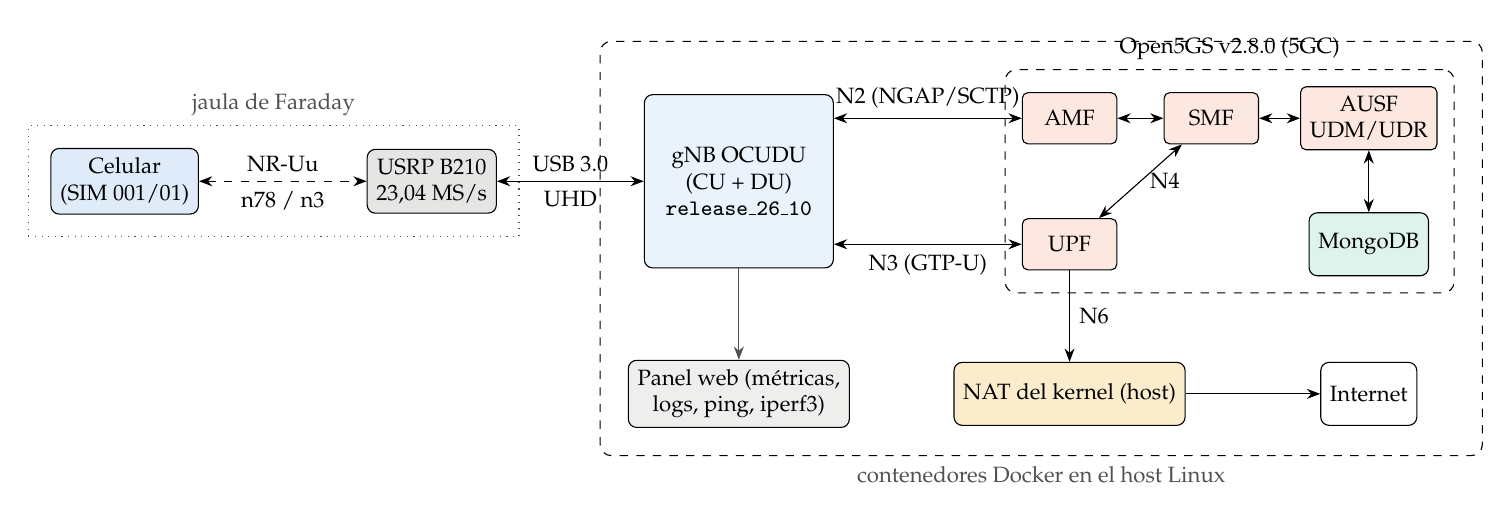
\begin{tikzpicture}[font=\footnotesize,>=Stealth,
  c/.style={draw,rounded corners=3pt,fill=white,minimum height=0.8cm,align=center},
  nf/.style={draw,rounded corners=2pt,fill=naranja!15,minimum width=1.2cm,minimum height=0.65cm,align=center}]
  \node[c,fill=azul!15] (ue) at (0,0) {Celular\\(SIM 001/01)};
  \node[c,fill=gris!15] (usrp) at (3.9,0) {USRP B210\\23,04 MS/s};
  \draw[<->,dashed] (ue) -- node[above]{NR-Uu} node[below]{n78 / n3} (usrp);
  \node[draw,dotted,gris,fit=(ue)(usrp),inner sep=8pt,label={[gris]above:jaula de Faraday}] {};
  \node[c,fill=azul!10,minimum width=2.4cm,minimum height=2.2cm] (gnb) at (7.8,0) {gNB OCUDU\\(CU + DU)\\\texttt{release\_26\_10}};
  \draw[<->] (usrp) -- node[above]{USB 3.0} node[below]{UHD} (gnb);
  \node[nf] (amf) at (12.0,0.8) {AMF};
  \node[nf] (smf) at (13.8,0.8) {SMF};
  \node[nf] (aus) at (15.8,0.8) {AUSF\\UDM/UDR};
  \node[nf] (upf) at (12.0,-0.8) {UPF};
  \node[c,fill=verde!15] (mongo) at (15.8,-0.8) {MongoDB};
  \draw[<->] (gnb.east |- amf) -- node[above]{N2 (NGAP/SCTP)} (amf);
  \draw[<->] (gnb.east |- upf) -- node[below]{N3 (GTP-U)} (upf);
  \draw[<->] (amf) -- (smf); \draw[<->] (smf) -- node[right]{N4} (upf);
  \draw[<->] (smf) -- (aus); \draw[<->] (aus) -- (mongo);
  \node[draw,dashed,rounded corners,fit=(amf)(smf)(upf)(aus)(mongo),inner sep=6pt,label={above:Open5GS v2.8.0 (5GC)}] (core) {};
  \node[c,fill=ocre!20] (nat) at (12.0,-2.7) {NAT del kernel (host)};
  \node[c] (inet) at (15.8,-2.7) {Internet};
  \draw[->] (upf) -- node[right]{N6} (nat); \draw[->] (nat) -- (inet);
  \node[c,fill=gris!10] (dash) at (7.8,-2.7) {Panel web (métricas,\\logs, ping, iperf3)};
  \draw[->,gris] (gnb) -- (dash);
  \node[draw,dashed,rounded corners,fit=(gnb)(core)(dash),inner sep=10pt,label={[gris]below:contenedores Docker en el host Linux}] {};
\end{tikzpicture}}
\caption{Arquitectura implementada. El celular y la antena de la B210 están dentro de la jaula de Faraday; el gNB, el núcleo, la base de datos y el panel de monitoreo corren en contenedores. La salida a Internet es por NAT del kernel del host.}
\label{fig:arquitectura}
\end{figure}

\subsection{Equipamiento y software}
\begin{table}[htbp]
\centering
\caption{Equipamiento y software.}
\label{tab:equipos}
\begin{tabularx}{\linewidth}{lX}
\toprule
Componente & Detalle \\
\midrule
Radio & USRP B210 sin GPSDO, por USB~3.0. 23,04~MS/s, formato \texttt{sc12}. Ganancia de TX 80~dB y de RX 40~dB. 1 antena de transmisión y 1 de recepción (1~capa) \\
gNB & OCUDU (ex srsRAN Project), versión \texttt{release\_26\_10}, en Docker \\
Núcleo & Open5GS v2.8.0 con MongoDB, en Docker \\
Salida a Internet & NAT del kernel Linux (N6) \\
PC principal & Intel i3-1005G1 (2 núcleos, 4 hilos), 7,3~GiB de RAM, Debian~13 \\
PC secundaria & PC del laboratorio con 12 hilos y 60~GiB de RAM \\
Teléfonos & Xiaomi Redmi Note~14~5G (el medido), OnePlus~13, Motorola Edge~30~Neo \\
SIM & Programables de laboratorio. Lista de PLMN y tecnologías de acceso grabadas por el grupo con comandos APDU desde Linux; claves, con la herramienta del fabricante \\
Monitoreo & Panel web propio en un contenedor sin privilegios: métricas y logs del gNB, ping e iperf3 \\
\bottomrule
\end{tabularx}
\end{table}

\subsection{Parámetros de la celda}
\begin{table}[htbp]
\centering
\caption{Parámetros de las dos celdas.}
\label{tab:celda}
\begin{tabular}{lll}
\toprule
Parámetro & Celda principal (n78) & Celda n3 \\
\midrule
Duplexado & TDD & FDD \\
Rango & FR1 & FR1 \\
NR-ARFCN DL & 635\,000 (3525~MHz) & 368\,500 (1842,5~MHz) \\
Frecuencia UL & 3525~MHz & 1747,5~MHz \\
SSB (ARFCN / GSCN) & 634\,656 / 7860 & 368\,410 / 4604 \\
Ancho de canal & 20~MHz & 20~MHz \\
Numerología & $\mu=1$, 30~kHz & $\mu=0$, 15~kHz \\
PRB & 51 & 106 \\
FFT a 23,04~MS/s & 768 & 1536 \\
PLMN / TAC / PCI & 001/01 / 7 / 1 & 001/01 / 7 / 1 \\
Patrón TDD & 5~ms: 6~D, 1~S (8~D + 6~G), 3~U & --- \\
PRACH & índice 159 (B4), $L_\text{RA}=139$, 30~kHz & índice 1 \\
Forma de onda & DL CP-OFDM; UL CP-OFDM & ídem \\
Modulación máxima DL & 256QAM & 256QAM \\
\bottomrule
\end{tabular}
\end{table}

\subsection{Decisiones de diseño justificadas}
\begin{itemize}
  \item \textbf{Banda n78 y 3525~MHz.} n78 es la banda media característica de 5G y la de la configuración de referencia del gNB para TDD. Primero se usó 3489,42~MHz, pero esa frecuencia cae en el bloque de un operador comercial y atraía a celulares ajenos. Por eso se pasó a 3525~MHz (ARFCN 635\,000, múltiplo del raster de 30~kHz de n78).
  \item \textbf{20~MHz y 30~kHz.} 20~MHz exige 23,04~MS/s, un caudal que la B210 sostiene por USB~3.0 y que la CPU disponible puede procesar; anchos mayores multiplican ambos (\cref{sec:fs}). 30~kHz es la SCS típica de n78 y deja un CP de 2,34~$\mu$s, sobrado para la jaula (\cref{sec:cp}).
  \item \textbf{Frecuencia de muestreo de 23,04~MS/s.} Es la mínima que contiene las 612 subportadoras con una FFT eficiente (768 puntos) y reduce en un 25~\% el caudal de muestras por USB frente a 30,72~MS/s (\cref{sec:fs}). Es de esperar que también baje la carga de CPU, pero no se midió.
  \item \textbf{Patrón TDD de 5~ms DDDDDDSUUU.} Es el patrón que el gNB usa por defecto, con predominio de la bajada (65,7~\%), adecuado para navegación. El slot especial deja 6 símbolos de guarda (214~$\mu$s), mucho más que lo que hace falta en la jaula.
  \item \textbf{PRACH formato B4 (índice 159).} Es el valor que el gNB usa por defecto para esta configuración. Es un formato corto (139 subportadoras de 30~kHz, igual a la SCS de los datos), sin largos preámbulos de 1,25~kHz que exigirían otra numerología en el PRACH. Ocupa un único slot de subida por trama y su alcance geométrico orientativo es de $\approx 2$~km (\cref{sec:ta}), más que suficiente para la jaula.
  \item \textbf{PLMN de prueba 001/01.} Con el PLMN 722/999 los teléfonos no generaban PRACH. El MCC~001 corresponde a redes de prueba, según la numeración de la Recomendación UIT-T E.212; solo se pudo contrastar con fuentes secundarias \verif, y con él los teléfonos se registraron (\cref{sec:crono}).
  \item \textbf{1 TX y 1 RX.} La B210 tiene dos cadenas, pero con dos antenas se duplican el caudal por USB y la carga de procesamiento. Con una sola capa la configuración es más simple y la referencia teórica (71,7~Mbit/s) alcanza para los objetivos del trabajo.
  \item \textbf{CP-OFDM en la subida.} Se probó DFT-s-OFDM y no mejoró el rendimiento en estas condiciones (\cref{sec:dfts,sec:crono}).
\end{itemize}

\subsection{SIM de laboratorio}
La lista de PLMN con tecnología de acceso (con el bit de NG-RAN activado) y el PLMN se grabaron desde Linux con comandos APDU \cite{ts31102}. Las claves del abonado ($K$ y OPc) se grabaron con la herramienta del fabricante de las tarjetas. La implementación de Milenage se contrastó con los vectores de prueba de TS~35.208 \cite{ts35208}, lo que valida el algoritmo pero no que las claves coincidan. Que coincidían entre las tarjetas y el núcleo se comprobó aparte, con un comando de autenticación a cada SIM, y finalmente con el registro exitoso. Las claves no se incluyen en este informe.

\section{Desarrollo cronológico: problemas detectados y soluciones}\label{sec:crono}

Esta sección relata el trabajo en el orden en que se hizo; la \cref{tab:evidencia} indica dónde está la evidencia de cada etapa. Para cada problema se presentan el síntoma observado, la explicación teórica y la solución adoptada. Las hipótesis que no pudieron demostrarse se señalan como tales.

\begin{table}[htbp]
\centering
\caption{Evidencia de cada etapa (carpetas del repositorio del grupo). Los identificadores de terceros están anonimizados.}
\label{tab:evidencia}
\begin{tabularx}{\linewidth}{lXX}
\toprule
Etapa & Evidencia & Qué muestra \\
\midrule
1. Sincronización & \texttt{evidencia/01\_sincronizacion} & Arranque del gNB, SSB, MIB/SIB1 y TDD \\
2. Acceso & \texttt{evidencia/02\_acceso} & PRACH y acceso de teléfonos con SIM de laboratorio y comercial \\
3. Registro & \texttt{evidencia/03\_registro} & NG Setup, registro y RLF por CSI \\
4. Sesión PDU & \texttt{evidencia/04\_sesion\_pdu} & Sesiones PDU, cortes de 60~s, logcat del módem y corridas con ``NR only'' \\
5. Tráfico IP & (en los logs de la etapa 4) & Primera navegación por NAT \\
6. Mediciones & \texttt{evidencia/06\_mediciones} & Prueba A/B/A, iperf3 y ping. Los JSON de iperf3 y la salida del ping no se conservaron: los valores son una transcripción hecha durante la sesión \\
\bottomrule
\end{tabularx}
\end{table}

\subsection*{Antecedente}
Una prueba previa de otro grupo había funcionado de punta a punta con un UE simulado por software y un enlace de radio también simulado. Por aire, en cambio, solo un celular comercial ajeno a la prueba había llegado al núcleo. Ese antecedente atribuía el fracaso a que las SIM no tenían el directorio de 5G (DF\_5GS). El grupo tomó esa conclusión como hipótesis a verificar, no como un hecho.

\subsection{30/10: entorno, contenedores y primera celda}
\paragraph{1. La B210 en USB~2.0.} Al conectarse, la B210 se enumeraba como dispositivo USB~2.0, y recién después de cargarle el firmware pasaba a USB~3.0 (5~Gb/s). Como 23,04~MS/s en \texttt{sc12} exigen $\approx 69$~MB/s en cada sentido (\cref{sec:fs}), más de lo que USB~2.0 sostiene en la práctica, se adoptó como procedimiento cargar el firmware después de cada conexión y verificar la velocidad del enlace antes de arrancar la celda.

\paragraph{2. Imágenes Docker y NG Setup.} Se construyeron las imágenes del gNB, del núcleo y de un UE simulado. El gNB y el AMF completaron el \emph{NG Setup} por la interfaz N2, lo que validó la conectividad SCTP entre contenedores y la coherencia del PLMN y el TAC entre el gNB y el núcleo.

\paragraph{3. Prueba con UE simulado, abandonada.} La prueba sin radio, con UE simulado y enlace por software, no avanzó. Además, el UE simulado solo admite una SCS de 15~kHz y no servía para la celda n78 a 30~kHz. El grupo la abandonó y pasó directamente a la celda real.

\paragraph{4. Primera celda por aire.} En la jaula se levantó la celda n78 en 3525~MHz. Antes se había usado 3489,42~MHz, pero esa frecuencia caía en el bloque de un operador comercial y atraía celulares ajenos.
\begin{itemize}
  \item El Redmi completó un registro una sola vez, sin sesión PDU.
  \item El Motorola con SIM de laboratorio no generó ningún PRACH.
  \item Con un chip comercial, el Motorola llegó al núcleo y fue rechazado, como se esperaba.
\end{itemize}

\paragraph{5. Conclusión de la etapa.} Que un teléfono con chip comercial llegara al núcleo muestra que la cadena de bajada y de acceso funcionaba al menos para ese teléfono: SSB, MIB, SIB1, PRACH, RAR, RRC y NGAP. Eso apoya la hipótesis de que el problema estaba en cómo trataba el teléfono a la SIM de laboratorio. La hipótesis del antecedente quedó \textbf{refutada}: una SIM sin DF\_5GS se registró.

\subsection{02/11: SIM, PLMN y primera navegación}
\paragraph{6. Sin PRACH con el PLMN 722/999.} Aun con el bit de NG-RAN grabado en la lista de PLMN y tecnologías de acceso de la SIM, los teléfonos no generaban ningún PRACH con el PLMN 722/999: 0 preámbulos en 2 minutos. Según la \cref{sec:encendido}, el UE solo inicia el acceso aleatorio si el PLMN difundido en el SIB1 le resulta aceptable. La ausencia de preámbulos detectados apoya la hipótesis de que el módem descartaba la celda antes del acceso, en la selección de PLMN o de celda; por sí sola no excluye un problema de detección, pero con 001/01 y la misma radio los teléfonos sí accedieron. Se cambió al PLMN de prueba 001/01, regrabando las SIM y el núcleo, y el Redmi se registró al primer intento. El OnePlus también. No se pudo identificar la causa dentro del módem.

\paragraph{7. Falla de enlace por CSI.} Con el CSI periódico, el gNB declaraba una falla de enlace (RLF) a los 3~s: había 100 reportes de CSI sin decodificar. Ese criterio de RLF es propio de la implementación del gNB: cuenta las recepciones fallidas consecutivas del PUCCH. No es el procedimiento de RLF del UE (T310/N310, \cite[§5.3.10]{ts38331}\verif). Se pasó al CSI aperiódico. Pero sin CSI-RS se perdía también el TRS, y la conexión empeoraba: como se explicó en la \cref{sec:pilotos}, NR no tiene una CRS siempre presente, y el TRS es la referencia con la que el UE corrige finamente tiempo y frecuencia.

\paragraph{8. Primera navegación.} Con esa configuración, el Redmi descargó $\approx 27$~MB por NAT, y el OnePlus obtuvo IP. Fue el primer camino completo: registro, sesión PDU, IP y tráfico.

\paragraph{9. Cortes cada 18--65~s.} La conexión se cortaba cada 18 a 65~s. Entre el 73 y el 92~\% de los PUSCH tenían error. Al abrir un navegador en la PC aparecían fallas de tiempo real ($\approx 900$ por minuto), y una vez la B210 perdió la conexión USB. En una radio definida por software, cada slot de 0,5~ms tiene un plazo estricto: si el procesamiento no llega a tiempo (\emph{late}) o el buffer de transmisión se vacía (\emph{underflow}), se transmiten o reciben símbolos incompletos y las transmisiones fallan. El problema quedó abierto.

\subsection{03/11, mañana: una PC más potente}
\paragraph{10. La CPU no era la causa principal.} En la segunda PC (12 hilos), el patrón fue el mismo, con el gNB usando $\approx 110~\%$ sobre 1200~\%. Por minuto hubo $\approx 130$ transmisiones de bajada que agotaron los 4 reintentos HARQ, $\approx 80$ fallas de tiempo real (\emph{late} y \emph{underflow}) y $\approx 2$ RLF. La bajada fallaba bastante más de lo que explicaban las fallas de tiempo real, y la CPU estaba casi libre en promedio (no se descarta que algún hilo crítico se saturara). \textbf{La CPU dejó de considerarse la causa principal}: el problema apuntaba a la radio o a la sincronización.

\paragraph{11. Configuración equivocada.} El script de arranque cargaba una configuración vieja. Se corrigió pasando la configuración como argumento y verificando qué archivo quedaba montado en el contenedor antes de cada prueba.

\subsection{03/11, tarde: las tres causas de los cortes}
\paragraph{12. Corrección de reloj (\texttt{clock\_ppm}).}
\textbf{Síntoma.} El gNB enviaba comandos de TA positivos sin parar, de $+2{,}2$ a $+3{,}8$ pasos de 0,26~$\mu$s por segundo, y las conexiones duraban de 3 a 10~s.

\textbf{Causa.} El grupo la verificó en el código del gNB: el parámetro \texttt{clock\_ppm} ($-1{,}87$~ppm, heredado del antecedente) corregía la frecuencia de portadora, pero no la de muestreo.

\textbf{Modelo explicativo propuesto.} Lo verificado es el efecto de \texttt{clock\_ppm} en el código y la mejora al anularlo; el mecanismo siguiente es la explicación que propone el grupo, porque no se pudo observar cómo acopla el módem del teléfono la corrección de frecuencia y la de tiempo. En la B210 sin referencia externa, la portadora y el reloj de muestreo derivan del mismo oscilador de referencia. Si este tiene un error relativo $\varepsilon$, ambos se desvían en la misma proporción:
\begin{equation}
f_c' = f_c(1+\varepsilon),\qquad f_s' = f_s(1+\varepsilon).
\end{equation}
Un teléfono también deriva portadora y muestreo de un único oscilador. Se sincroniza a la portadora que recibe (corrige el CFO con el PSS, el SSS y el TRS) y, al hacerlo, su reloj de muestreo queda escalado en la misma proporción. Si los dos extremos tienen un oscilador común, la base de tiempo que deduce el UE de la portadora coincide con la del gNB.

Al aplicar la corrección solo a la portadora, ese vínculo se rompe: la portadora del gNB queda desplazada en $\delta = 1{,}87$~ppm respecto de lo que implica su reloj de muestreo. El UE ajusta su oscilador a la portadora corregida, y su base de tiempo queda desfasada $\delta$ respecto de la del gNB. La temporización relativa deriva a razón de
\begin{equation}
\dot{\tau} = \delta = 1{,}87\cdot 10^{-6}~\text{s/s} = 1{,}87~\mu\text{s por segundo} \approx \frac{1{,}87~\mu\text{s}}{0{,}260~\mu\text{s}} \approx 7~\text{pasos de TA por segundo}.
\end{equation}
Es del mismo orden que lo observado (2,2 a 3,8 pasos por segundo, es decir, 0,6 a 1,0~$\mu$s/s), aunque no coincide: el modelo no explica el valor exacto, que depende de cómo el módem reparte la corrección entre la bajada y la subida. El gNB ve llegar la subida cada vez más tarde y responde con comandos de TA (\cref{sec:ta}, \cite[§4.2]{ts38213}). Si la corrección se retrasa, el error de temporización supera el CP de 2,34~$\mu$s en pocos segundos: aparece ISI, los PUSCH fallan y la conexión cae. Eso coincide con los cortes a los 3--10~s.

En frecuencia, la corrección configurada de 1,87~ppm desplazaba la portadora $1{,}87\cdot 10^{-6}\cdot 3525~\text{MHz}\approx 6{,}6$~kHz, el 22~\% de la SCS. Ese valor es el de la corrección, no una medición del error real del oscilador de la B210.

\textbf{Solución.} Con \texttt{clock\_ppm} = 0, portadora y muestreo vuelven a tener el mismo error relativo y el UE los sigue juntos. El TA quedó estable y las conexiones pasaron a durar $\approx 60$~s.

\paragraph{13. El Redmi no envía CSI.} De $\approx 10\,000$ pedidos de CSI aperiódico (por PUSCH), el gNB no decodificó ninguno. Del CSI periódico por PUCCH formato~2 se decodificó solo el $\approx 0{,}4~\%$. El OnePlus sí lo enviaba, lo que apoya que el comportamiento era propio del Redmi, aunque no demuestra que la configuración fuera la ideal para él. Se volvió al CSI periódico, que mantiene los CSI-RS y el TRS, y se elevó mucho el umbral de recepciones fallidas consecutivas del PUCCH del gNB. Así, el CSI faltante ya no dispara RLF, a costa de que el gNB elija el MCS sin CQI, solo con el HARQ.

\paragraph{14. Corte casi exacto cada 60~s.} Con los dos cambios anteriores, la conexión se cortaba casi exactamente cada 60~s, tanto en n78 TDD como en n3 FDD. En esta etapa, la celda \textbf{n3 FDD funcionó por primera vez}.
\begin{itemize}
  \item Con los registros del módem (\texttt{adb logcat}) se vio que el Redmi perdía el servicio entre 59,99 y 60,02~s después de obtenerlo, en 5 ciclos, sin una liberación previa de la red. Después buscaba LTE comercial.
  \item Un período tan exacto y el mismo en dos bandas y dos duplexados apunta a un temporizador del teléfono o del protocolo más que a una causa de radio, aunque no la descarta del todo.
  \item \textbf{Hipótesis principal (no demostrada):} el núcleo anuncia soporte de voz sobre IMS (\emph{IMS voice over PS}~=~1, en el IE \emph{5GS network feature support} del Registration Accept \cite[§9.11.3.5]{ts24501}\verif) sin tener un IMS. Un UE configurado como \emph{voice centric}, que no consigue servicio de voz en 5GS, abandona 5G y busca E-UTRA \cite[§4.3.2]{ts24501}\verif. Los 60~s serían el tiempo que este módem espera el registro IMS antes de rendirse; la norma no fija un temporizador universal de 60~s para esto.
  \item \textbf{Mitigación:} se activaron VoLTE y el tipo de red ``NR only'' en el teléfono. Con eso, el Redmi se mantuvo conectado 5~min~39~s en n3, donde la sesión terminó por una RLF, y 5~min~45~s en n78, sin RLF, hasta que se detuvo el gNB.
\end{itemize}

\paragraph{15. Quedaron abiertos.}
\begin{itemize}
  \item El OnePlus no permite forzar ``NR only'' desde el menú y se corta a los $\approx 35$--37~s. Pide la DNN \texttt{ims}, lo que es coherente con la hipótesis de voz.
  \item Una falla de tiempo real del gNB, ``UL processor is busy''.
\end{itemize}

\subsection{03/11, noche: monitoreo, DFT-s-OFDM y mediciones}
\paragraph{16. Panel de monitoreo.} El grupo armó un panel web en un contenedor sin privilegios. Lee las métricas y los logs del gNB, y lanza ping e iperf3 hacia el teléfono, sin tocar la configuración de la celda.

\paragraph{17. ``UL processor is busy''.}
\begin{itemize}
  \item Aparece después de ráfagas de fallas de tiempo real y persiste hasta que se detiene la celda, a razón de 10 a 60 por segundo.
  \item Cae en los slots de subida (7, 8, 9, 17, 18 y 19), sobre todo en el 19, que es el del PRACH (\cref{fig:tdd}).
  \item Ocurrió en 2 de 3 corridas y degrada la celda.
\end{itemize}
Que se concentre en el slot~19 tiene una posible explicación teórica, que el grupo deja como \textbf{hipótesis a verificar}. Con $N_\text{CS}=0$ (\cref{sec:rach}), los 64 preámbulos salen de 64 raíces ZC distintas. Un detector que correlaciona en frecuencia obtiene \emph{todos} los desplazamientos cíclicos de una raíz con una sola correlación, pero necesita una por raíz. Además, en el formato B4 el preámbulo se repite 12 veces. El procesamiento del slot del PRACH sería, entonces, el más pesado de la trama, y el primero en atrasarse después de una perturbación.

La mitigación adoptada fue medir con la celda recién arrancada, poner el governor de la CPU en \texttt{performance} y no ejecutar aplicaciones pesadas durante las mediciones. La causa de fondo quedó abierta.

\paragraph{18. Prueba A/B/A de la forma de onda de subida.} Se comparó CP-OFDM con DFT-s-OFDM en la subida, con el Redmi y subidas TCP de 10~s, alternando la configuración A, B, A para detectar derivas (\cref{tab:aba}).

\begin{table}[htbp]
\centering
\caption{Prueba A/B/A de la forma de onda de subida (subida TCP de 10~s, Redmi). Una corrida de la celda por tramo.}
\label{tab:aba}
\begin{tabular}{llcccc}
\toprule
Tramo & UL & Promedio [Mbit/s] & Desvío [Mbit/s] & Pruebas & SINR PUSCH media \\
\midrule
A1 & CP-OFDM & 8,66 & 0,40 & 2 & $\approx 19$~dB \\
B & DFT-s-OFDM & 12,70 & 1,35 & 4 & $\approx 27$~dB \\
A2 & CP-OFDM & 14,84 & 1,18 & 4 & $\approx 27$~dB \\
\bottomrule
\end{tabular}
\end{table}

\begin{itemize}
  \item \textbf{DFT-s-OFDM funciona:} los dos teléfonos entraron a la celda, y se usó 256QAM con transform precoding. La asignación máxima fue de 50~PRB, como exige la \cref{eq:235}.
  \item \textbf{No mejoró el rendimiento.} B quedó entre A1 y A2. Con la misma SINR ($\approx 27$~dB), A2 superó a B en $\approx 2{,}1$~Mbit/s. Parte de la diferencia puede deberse a la asignación (50 contra 51~PRB: un 2~\%). El resto no se puede separar de la variabilidad entre corridas, de la implementación del receptor ni de las condiciones no controladas: la prueba no permite atribuirlo a la forma de onda.
  \item \textbf{Interpretación.} Con SINR alta y un UE sin limitación de potencia (\cref{sec:potencia_ul}), la menor PAPR de DFT-s-OFDM no aporta nada: su beneficio aparece en el borde de la celda, cuando el amplificador del UE trabaja cerca de la saturación. Es una \textbf{hipótesis}, porque no se registró el PHR que la confirmaría. Por eso se mantuvo CP-OFDM.
  \item A1 tuvo peor enlace (SINR $\approx 19$~dB) por una causa no identificada. Hubo una sola corrida por tramo, así que la prueba no permite separar el efecto de la forma de onda de la variabilidad entre corridas.
\end{itemize}

\paragraph{19. Bajada TCP de 10~s (tramo A2).} Se midió con iperf3 en modo inverso: el servidor, en el panel, transmitía hacia el teléfono, y el valor informado es la tasa del emisor, no el goodput recibido. Se obtuvieron 55,2, 52,7 y 42,2~Mbit/s. La tercera coincidió con la aparición de ``UL processor is busy''. Con la celda limpia, la bajada fue de $\approx 54$~Mbit/s.

\paragraph{20. Ping al teléfono, con la celda ya degradada.} El RTT mínimo fue de 16,7~ms, el mediano de 27,7~ms, el percentil 90 de 44,9~ms y el máximo de 1052~ms, con un 21,7~\% de pérdida (60 paquetes enviados cada 0,5~s, 47 recibidos) y un jitter de 52,3~ms, calculado como la media de las diferencias entre RTT sucesivos (no es jitter unidireccional). Como la celda ya presentaba ``UL processor is busy'', es el resultado de una sola corrida degradada y hay que repetirlo con la celda limpia.

\section{Resultados y análisis frente a la teoría}\label{sec:resultados}

\subsection{Resumen de mediciones}
La \cref{tab:resultados} reúne las mediciones de la celda n78 con el Redmi en ``NR only'' y las compara con las referencias aproximadas de la \cref{sec:tput}. Las mediciones TCP duran 10~s y son una transcripción hecha durante la sesión: no se conservaron los archivos originales de iperf3 ni del ping.

\begin{table}[htbp]
\centering
\caption{Mediciones de la celda n78 frente a la teoría.}
\label{tab:resultados}
\begin{tabular}{lccc}
\toprule
Magnitud & Medido & Teórico (TS~38.306) & Medido/teórico \\
\midrule
Bajada TCP (celda limpia, tasa del emisor) & $\approx 54$~Mbit/s & 71,7~Mbit/s & 75~\% \\
Subida TCP (CP-OFDM, A2) & 14,8~Mbit/s & 35~Mbit/s (26 con 64QAM) & 42~\% (57~\%) \\
Subida TCP (DFT-s-OFDM, B) & 12,7~Mbit/s & 34,3~Mbit/s (50~PRB) & 37~\% \\
RTT mín. / mediano$^\dagger$ & 16,7 / 27,7~ms & --- & --- \\
RTT p90 / máx.$^\dagger$ & 44,9 / 1052~ms & --- & --- \\
Jitter$^\ddagger$ / pérdida$^\dagger$ & 52,3~ms / 21,7~\% & --- & --- \\
\bottomrule
\multicolumn{4}{l}{\footnotesize $^\dagger$ Con la celda ya degradada por ``UL processor is busy''; una sola corrida.}\\
\multicolumn{4}{l}{\footnotesize $^\ddagger$ Media de las diferencias entre RTT sucesivos.}
\end{tabular}
\end{table}

\subsection{Bajada: 75~\% de la referencia teórica}
Los $\approx 54$~Mbit/s representan el 75~\% de los 71,7~Mbit/s de la \cref{eq:dlmax}. La eficiencia espectral efectiva es $54/20 = 2{,}7$~bit/s/Hz, contra $71{,}7/20 = 3{,}6$~bit/s/Hz teóricos. La diferencia se explica por varios factores:
\begin{itemize}
  \item \textbf{MCS no siempre máximo:} solo el 72,6~\% de los PDSCH usó 256QAM (\cref{tab:modulaciones}), y no siempre con el MCS~27.
  \item \textbf{Retransmisiones HARQ:} cada TB que falla ocupa un slot sin aportar datos nuevos.
  \item \textbf{Overhead real distinto del 14~\% supuesto:} SSB, CSI-RS y TRS, PDCCH, DM-RS y los slots del SIB1 y del paging.
  \item \textbf{TCP:} el control de congestión no mantiene el enlace lleno todo el tiempo, y sus ACK viajan por la subida, que es más lenta y tiene más latencia.
\end{itemize}
Con todo, alcanzar el 75~\% de la referencia con una radio definida por software y una sola antena es compatible con que la cadena de bajada (sincronización, estimación de canal, LDPC y 256QAM) funcione según lo previsto.

\subsection{Asimetría bajada/subida}
La bajada fue $54/14{,}8\approx 3{,}6$ veces más rápida que la subida. La teoría explica esta asimetría con tres causas:
\begin{enumerate}
  \item \textbf{Patrón TDD:} el 65,7~\% de los símbolos es de bajada y solo el 30~\% de subida (\cref{eq:fdl,eq:ful}). Esto solo ya explica un factor de 2,2.
  \item \textbf{Potencia:} el gNB reparte su potencia sobre una EPRE constante (\cref{sec:potencia_dl}), mientras que el UE ajusta la suya en lazo abierto y cerrado para llegar a una densidad objetivo (\cref{sec:potencia_ul}). La SINR del PUSCH no la elige el UE, sino el control de potencia, y la subida también sufre los errores de temporización y la carga de procesamiento del receptor del gNB.
  \item \textbf{Acceso planificado:} cuando el UE no tiene un grant vigente, una nueva ráfaga de subida necesita el ciclo SR $\to$ grant $\to$ PUSCH, con $k_2\ge 4$ slots (\cref{sec:grant}); con tráfico sostenido, los BSR mantienen los grants sin nuevos SR. En la bajada, el gNB planifica directamente.
\end{enumerate}

\subsection{Subida medida contra teórica}
Los 14,8~Mbit/s son el 42~\% del máximo de 35~Mbit/s (57~\% si se toma como referencia 64QAM). Las causas probables son:
\begin{itemize}
  \item \textbf{Errores de PUSCH y BLER:} el PUSCH tuvo más fallas en la primera transmisión. Cada fallo exige una retransmisión, que en TDD solo puede ir en un slot de subida, a menudo del período siguiente.
  \item \textbf{Planificación por SR/BSR:} el gNB solo asigna lo que el BSR le informa, y con un retardo de varios slots. Si el buffer del UE se vacía entre grants, quedan slots de subida sin usar.
  \item \textbf{Dinámica de TCP:} la ventana de congestión crece según los ACK, que llegan con el RTT del enlace. Con un RTT de decenas de milisegundos y pérdidas por errores de radio, TCP no llega a llenar el canal en 10~s.
  \item \textbf{Recursos compartidos en los slots de subida:} el PUCCH, el PRACH del slot~19 y la carga del procesador de subida reducen los PRB y los slots útiles para el PUSCH.
\end{itemize}

\subsection{Latencia y TDD}\label{sec:latencia}
El RTT mínimo de 16,7~ms es coherente con la estructura de la celda. Un ping recorre la bajada y la subida, y cada sentido tiene sus esperas. Las siguientes son estimaciones de orden de magnitud para un UE sin grant vigente; dependen del período y el desfase de las ocasiones de SR, que no se relevaron:
\begin{itemize}
  \item \textbf{Bajada:} el paquete espera un slot de bajada (en promedio, poco, porque son el 65,7~\% del tiempo). Después, el PDSCH y el HARQ-ACK, que espera un slot de subida.
  \item \textbf{Subida (la respuesta):} el UE tiene que esperar una ocasión de SR en un slot de subida. Los slots de subida están agrupados al final de cada período de 5~ms, así que la espera hasta el próximo es del orden de algunos milisegundos. Después, el grant en un slot de bajada y el PUSCH $k_2\ge 4$ slots más tarde, que en la práctica cae en el período de subida siguiente: $\approx 5$~ms más.
\end{itemize}
Sumando el procesamiento del gNB, el UPF y el teléfono, una decena de milisegundos de RTT solo por la interfaz radio es plausible, y el mínimo medido está en ese orden. Si el teléfono entra en DRX entre pings, a esto se suma la espera hasta el próximo \emph{on duration} (\cref{sec:callado}). La mediana (27,7~ms), el jitter (52,3~ms), el máximo de 1052~ms y la pérdida del 21,7~\% no son representativos de la tecnología: se midieron con el procesador de subida del gNB saturado (``UL processor is busy''), que descarta subidas enteras. Por eso deben repetirse con la celda limpia.

\subsection{Comparación con 2G y 4G}
La \cref{tab:comparacion} queda preparada para la comparación con las mediciones de EDGE y LTE del mismo grupo. La columna de NR tiene los valores de este trabajo.

\begin{table}[htbp]
\centering
\caption{Comparación entre tecnologías. Las columnas de EDGE y LTE se completan con las mediciones correspondientes.}
\label{tab:comparacion}
\begin{tabular}{lccc}
\toprule
Magnitud & EDGE (2G) & LTE (4G) & NR SA (este trabajo) \\
\midrule
Ancho de banda de canal & & & 20~MHz (n78, TDD) \\
Bajada TCP & & & $\approx 54$~Mbit/s (emisor) \\
Subida TCP & & & 14,8~Mbit/s \\
Referencia teórica DL / UL & & & 71,7 / 35~Mbit/s \\
RTT mínimo / mediano & & & 16,7 / 27,7~ms$^\dagger$ \\
Jitter & & & 52,3~ms$^\dagger$ \\
Pérdida de paquetes & & & 21,7~\%$^\dagger$ \\
\bottomrule
\multicolumn{4}{l}{\footnotesize $^\dagger$ Con la celda degradada; hay que repetirlo con la celda limpia.}
\end{tabular}
\end{table}

\section{Preguntas de la cátedra}\label{sec:preguntas}

Esta sección responde brevemente cada pregunta e indica dónde se desarrolla.

\paragraph{1. ¿Cómo son los flujos, cuántos bits por segundo y cuál es el peso de las palabras?}
Por cada slot asignado, la MAC entrega un bloque de transporte. Para 51~PRB, MCS~27 en 256QAM y una capa, el TBS es de 54\,296~bits (\cref{eq:tbs}), que con su CRC se segmentan en 7 code blocks LDPC del BG1: cada uno lleva 7760~bits del TB, 24 de CRC y 664 de relleno, es decir, 8448~bits de entrada al codificador ($Z_c=384$). Al ritmo de 2000 slots por segundo y con el 65,7~\% de símbolos de bajada, la referencia aproximada es de 71,7~Mbit/s en la bajada y $\approx 35$~Mbit/s en la subida. Se midieron $\approx 54$ y 14,8~Mbit/s (\cref{sec:flujos,sec:resultados}).

\paragraph{2. ¿Cómo se asigna el presupuesto de potencia?}
En la bajada, con el modelo simplificado de carga completa, el gNB reparte su potencia total con una EPRE aproximadamente constante sobre las 612~RE de cada símbolo ($-27{,}9$~dB respecto del total). En lugar de un lazo de potencia por usuario, se adapta el MCS con el CQI. Hay relaciones fijas o señalizadas entre la EPRE del PSS, el SSS, el CSI-RS y la DM-RS (\cref{sec:potencia_dl}). En la subida, cada UE fija su potencia con la \cref{eq:ppusch}: compensación fraccional de la pérdida de trayecto en lazo abierto, escalada con los PRB asignados y corregida en lazo cerrado con los comandos TPC, hasta $P_\text{CMAX}$. El PHR informa el margen (\cref{sec:potencia_ul}). El PRACH usa lazo abierto con rampa de potencia (\cref{eq:ramping}).

\paragraph{3. ¿Qué pasa apenas se prende el celular y en qué momento se engancha?}
El UE elige las bandas según la SIM y sus capacidades, recorre el sync raster (GSCN) buscando el PSS, se sincroniza en tiempo de símbolo y frecuencia gruesa con el PSS, obtiene el PCI con el SSS y se sincroniza a la trama al decodificar el PBCH (SFN e índice de SSB). Se ``engancha'' a la celda cuando decodifica el SIB1 y comprueba el PLMN y el nivel mínimo; recién entonces puede iniciar el RACH (\cref{sec:encendido}). En este trabajo, con el PLMN 722/999 el proceso se detenía antes del RACH (\cref{sec:crono}).

\paragraph{4. ¿Por qué se hace el scrambling?}
Para que la interferencia de otras celdas y de otros usuarios se vea como ruido después de la desaleatorización (la secuencia depende del PCI y del RNTI), para balancear los bits y evitar líneas espectrales, y, en el PBCH, para transportar información implícita del SFN y del SSB (\cref{sec:scrambling}).

\paragraph{5. ¿Por qué hay diferencia entre CP-OFDM y DFT-s-OFDM?}
DFT-s-OFDM antepone una DFT de $M$ puntos que convierte la señal en una portadora única interpolada: su envolvente sigue a la constelación y su PAPR es de 2,5 a 3,7~dB menor que la de CP-OFDM. Eso le permite al UE trabajar con menos back-off cuando está limitado en potencia. CP-OFDM admite MIMO y asignaciones flexibles, conserva la SINR de cada subportadora y suele rendir más con SINR alta (\cref{sec:dfts}). La prueba A/B/A fue coherente con eso: con SINR alta, DFT-s-OFDM no mejoró el rendimiento, aunque con una sola corrida por tramo (\cref{tab:aba}).

\paragraph{6. En OFDMA, ¿cuál tiene mayor PAPR y por qué crece con $N$?}
La señal con más subportadoras activas: en OFDMA, la del gNB, que suma las de todos los usuarios, y en general CP-OFDM frente a DFT-s-OFDM. No es que cada símbolo tenga más PAPR: cada muestra es aproximadamente gaussiana con la misma potencia media, independientemente de $N$. Al aumentar $N$ hay más muestras independientes por símbolo y \textbf{aumenta la probabilidad} de que alguna supere un umbral dado: $\Pr\{\text{PAPR}>\gamma_0\}\approx \alpha N e^{-\gamma_0}$ (\cref{eq:ccdf_aprox}). El umbral para una probabilidad fija crece como $\ln N$: de 9,7 a 11,7~dB al nivel $10^{-3}$ entre $N=16$ y $N=1024$ (\cref{sec:papr}, \cref{fig:papr}).

\paragraph{7. ¿Cuál es el valor mínimo del prefijo cíclico?}
El CP tiene que ser mayor que el delay spread del canal (más el error residual de sincronización): $T_\text{CP}\ge \tau_\text{max}$ (\cref{eq:cpmin}). Así la ISI queda dentro del CP y la convolución con el canal se vuelve circular. El ejercicio de la cátedra y su comparación con NR están en la \cref{sec:ejercicio_cp}. En la celda, 2,34~$\mu$s tolera $\approx 703$~m de diferencia de camino.

\paragraph{8. ¿Cuánto vale la frecuencia de muestreo en 5G?}
La norma define una unidad $T_c = 1/(480~\text{kHz}\cdot 4096)$, es decir, una ``frecuencia básica'' de 1,966~GHz que no se usa físicamente. Un equipo muestrea a $f_s = N_\text{FFT}\cdot\Delta f$. En esta celda, $f_s = 1536\times 15~\text{kHz} = 768\times 30~\text{kHz} = 23{,}04$~MS/s (\cref{sec:fs}, \cref{tab:fs}).

\paragraph{9. ¿Cómo se relaciona el timing advance con el radio de cobertura?}
El TA compensa el retardo de ida y vuelta: $d = c\,N_\text{TA}T_c/2$. Con $\mu=1$, cada paso es de 0,26~$\mu$s, unos 39~m, y el TA máximo de la RAR (1~ms) corresponde a $\approx 150$~km. El radio real lo limita el PRACH, que se transmite \emph{sin} TA: el retardo de ida y vuelta tiene que caber en el CP del preámbulo y en el tiempo de guarda. Para el formato B4 de la celda, eso da un alcance geométrico orientativo de $\approx 2$~km (\cref{sec:ta}).

\paragraph{10. En DFT-s-OFDM, ¿se ecualiza antes o después de la IDFT?}
\textbf{Antes.} En el receptor se ecualiza en frecuencia, después de la FFT de $N$ puntos y del demapeo de las $M$ subportadoras, y antes de la IDFT de $M$ puntos que deshace la precodificación. Ahí el canal es diagonal (un coeficiente por subportadora, gracias al CP), y después de la IDFT dejaría de serlo (\cref{sec:ecualizacion}, \cref{fig:dfts}).

\section{Conclusiones y trabajo futuro}\label{sec:conclusiones}

\subsection{Conclusiones}
\begin{enumerate}
  \item \textbf{Se cumplió el objetivo principal.} Una celda 5G NR SA (Release~15), implementada por completo en contenedores Docker con una USRP B210, registró un teléfono comercial con una SIM de laboratorio, le asignó una IP y le dio salida a Internet, tanto en n78 TDD como en n3 FDD.
  \item \textbf{La teoría de capa física explicó las decisiones de diseño.}
  \begin{itemize}
    \item La numerología y la frecuencia de muestreo ($1536\times 15$~kHz $=$ 23,04~MS/s) fijaron la FFT, el CP y el caudal por USB.
    \item El cálculo de PRB y guardas dio los 51 y 106~PRB.
    \item El análisis del formato B4 permitió estimar el alcance geométrico orientativo del PRACH.
  \end{itemize}
  \item \textbf{La sincronización fue el problema más difícil y el más instructivo.} Una corrección de reloj aplicada solo a la portadora, y no al muestreo, coincidía con una deriva constante del timing advance y con cortes a los pocos segundos; al anularla, el TA se estabilizó. El grupo lo explica porque se rompe el vínculo entre portadora y muestreo que el UE usa para mantener la temporización. Se detectó por la tendencia de los comandos de TA y se explicó con la teoría de TA de TS~38.213 §4.2.
  \item \textbf{Las señales piloto de NR son específicas.} Deshabilitar los CSI-RS eliminó también el TRS y empeoró el enlace, lo que es coherente con que, sin la CRS de LTE, el UE dependa del TRS para el seguimiento fino.
  \item \textbf{El rendimiento es compatible con la referencia teórica.} La bajada alcanzó el 75~\% de la referencia aproximada derivada de TS~38.306. La asimetría con la subida se explica con el patrón TDD, el acceso planificado y el control de potencia.
  \item \textbf{DFT-s-OFDM no es mejor en todos los casos.} Funcionó, pero con SINR alta no mejoró el throughput. Esto es coherente con el análisis probabilístico de la PAPR (su ventaja, de 2,5 a 3,7~dB en la simulación, importa cuando el UE está limitado en potencia), aunque que el Redmi no lo estuviera sigue siendo una hipótesis sin PHR.
  \item \textbf{Parte de los problemas no fueron de radio,} sino de la interacción del teléfono con la red: el PLMN no aceptado y el corte cada 60~s, que se mitigó con ``NR only'' y cuya relación con la voz IMS sigue siendo una hipótesis. Para un despliegue de laboratorio, la configuración del núcleo y de la SIM es tan importante como la de la capa física.
\end{enumerate}

\subsection{Trabajo futuro}\label{sec:trabajo_futuro}
\begin{itemize}
  \item Repetir el ping y la bajada con la celda recién arrancada, para obtener latencia, jitter y pérdida representativos.
  \item Identificar la causa de ``UL processor is busy''. Una prueba concreta, derivada de la \cref{sec:crono}: subir \texttt{zeroCorrelationZoneConfig} para que los 64 preámbulos salgan de pocas raíces ZC, y ver si la falla deja de concentrarse en el slot del PRACH.
  \item Confirmar la hipótesis de voz cambiando solo el anuncio de IMS en el núcleo, o montar un IMS.
  \item Forzar ``NR only'' en el OnePlus (por ejemplo, con los menús de prueba del módem).
  \item Repetir la comparación de DFT-s-OFDM en bloques alternados (ABAB/BABA), con más corridas y registrando el PHR, y en una condición de UE limitado en potencia (más atenuación o menos ganancia de recepción).
  \item Justificar formalmente el uso del PLMN de prueba 001/01 con la normativa de numeración.
  \item Completar la tabla comparativa con EDGE y LTE.
\end{itemize}

\begin{thebibliography}{99}
\bibitem{ts38101} 3GPP TS 38.101-1, \emph{NR; User Equipment (UE) radio transmission and reception; Part 1: Range 1 Standalone}, v15.31.0, Release 15.
\bibitem{ts38104} 3GPP TS 38.104, \emph{NR; Base Station (BS) radio transmission and reception}, Release 15.
\bibitem{ts38211} 3GPP TS 38.211, \emph{NR; Physical channels and modulation}, v15.10.0, Release 15.
\bibitem{ts38212} 3GPP TS 38.212, \emph{NR; Multiplexing and channel coding}, v15.13.0, Release 15.
\bibitem{ts38213} 3GPP TS 38.213, \emph{NR; Physical layer procedures for control}, v15.15.0, Release 15.
\bibitem{ts38214} 3GPP TS 38.214, \emph{NR; Physical layer procedures for data}, v15.16.0, Release 15.
\bibitem{ts38300} 3GPP TS 38.300, \emph{NR; NR and NG-RAN Overall Description; Stage 2}, Release 15.
\bibitem{ts38304} 3GPP TS 38.304, \emph{NR; User Equipment (UE) procedures in Idle mode and RRC Inactive state}, Release 15.
\bibitem{ts38306} 3GPP TS 38.306, \emph{NR; User Equipment (UE) radio access capabilities}, Release 15.
\bibitem{ts38321} 3GPP TS 38.321, \emph{NR; Medium Access Control (MAC) protocol specification}, v15.14.0, Release 15.
\bibitem{ts38331} 3GPP TS 38.331, \emph{NR; Radio Resource Control (RRC); Protocol specification}, v15.30.0, Release 15.
\bibitem{ts38133} 3GPP TS 38.133, \emph{NR; Requirements for support of radio resource management}, v15.35.0, Release 15.
\bibitem{ts23122} 3GPP TS 23.122, \emph{Non-Access-Stratum (NAS) functions related to Mobile Station (MS) in idle mode}, Release 15.
\bibitem{ts24501} 3GPP TS 24.501, \emph{Non-Access-Stratum (NAS) protocol for 5G System (5GS); Stage 3}, v15.7.0, Release 15.
\bibitem{ts31102} 3GPP TS 31.102, \emph{Characteristics of the Universal Subscriber Identity Module (USIM) application}, Release 15.
\bibitem{ts35208} 3GPP TS 35.208, \emph{Specification of the MILENAGE algorithm set; Document 4: Design conformance test data}.
\bibitem{vannee} R. van Nee y R. Prasad, \emph{OFDM for Wireless Multimedia Communications}, Artech House, 2000.
\bibitem{tanenbaum} A. S. Tanenbaum y D. J. Wetherall, \emph{Computer Networks}, 5.\textsuperscript{a} ed., Pearson, 2011.
\end{thebibliography}


\end{document}
